\documentclass[UTF8,12pt,a4paper]{ctexart}
\usepackage[a4paper,margin=2.5cm]{geometry}
\usepackage{enumitem}
\usepackage{hyperref}
\usepackage{graphicx}
\graphicspath{{assets/}}
\usepackage{float}
\usepackage{booktabs}
\usepackage{array}
\usepackage{tabularx}
\usepackage{fancyhdr}
\usepackage{xcolor}
\usepackage{listings}
\hypersetup{colorlinks=true,linkcolor=black,urlcolor=blue}
\setmainfont{Times New Roman}
\setCJKmainfont{Songti SC}
\setCJKsansfont{Heiti SC}
\setlength{\parindent}{2em}
\setlength{\parskip}{0.3em}
\setlist[itemize]{leftmargin=2em,itemsep=0.3em,topsep=0.3em}
\renewcommand{\arraystretch}{1.22}
\renewcommand{\tabularxcolumn}[1]{>{\raggedright\arraybackslash}p{#1}}
\newcolumntype{L}[1]{>{\raggedright\arraybackslash}p{#1}}
\renewcommand{\thefigure}{6-\arabic{figure}}
\renewcommand{\thetable}{6-\arabic{table}}
\lstset{
  language=Python,
  basicstyle=\ttfamily\scriptsize,
  breaklines=true,
  columns=fullflexible,
  keepspaces=true,
  extendedchars=true,
  inputencoding=utf8,
  frame=single,
  numbers=left,
  numberstyle=\tiny,
  keywordstyle=\color{blue!70!black},
  commentstyle=\color{green!35!black},
  stringstyle=\color{red!55!black},
  showstringspaces=false,
  captionpos=b,
  xleftmargin=2em,
}
\renewcommand{\lstlistingname}{代码}
\def\thelstlisting{6-\arabic{lstlisting}}
\sloppy
\pagestyle{fancy}
\fancyhf{}
\fancyfoot[C]{\thepage}
\renewcommand{\headrulewidth}{0pt}

\begin{document}
\renewcommand{\thelstlisting}{6-\arabic{lstlisting}}

\section*{实验6：工具调用、Agent与Harness实现}

\begin{center}
姓名：罗心月\qquad 学号：24111302025\qquad 班级：一班
\end{center}

\section*{1. 实验目的}

\begin{itemize}
  \item 掌握工具接口定义、参数验证、权限边界和结果反馈。
  \item 实现一个由模型根据任务和工具结果决定下一步操作、运行状态可查看且能够终止的单Agent。
  \item 编写运行时Harness，完成上下文组织、工具执行、结果检查、停止控制和日志记录。
\end{itemize}

\section*{2. 实验内容}

\subsection*{2.1 任务选择与边界}

\begin{itemize}
  \item 结合个人软件选择一个范围较小、结果能够检查的任务，如查询样例数据后生成统计结果；不适合接入个人软件时，可独立完成练习。
  \item 列出任务目标、可用数据、工具、停止条件和成功标准，并给出一组输入及预期结果。本实验实现单Agent，由模型根据目标和工具结果决定下一步操作；说明哪些步骤由程序预设，哪些由模型决定。
  \item 说明哪些操作允许自动执行，哪些必须用户确认，哪些明确禁止。
\end{itemize}

\subsection*{2.2 工具接口与参数约束}

\begin{itemize}
  \item 实现至少2个可实际运行的工具，如读取样例文件、查询数据或执行统计计算，说明名称、用途、输入字段、类型、必填项、返回结果和错误信息。输入格式及字段约束也称Schema。
  \item 建立允许调用的工具列表，执行前由程序检查工具名称、参数和访问范围，例如数值范围、允许的文件目录或可访问的数据；不能直接执行模型生成的任意函数名或命令。
  \item 说明工具的最长等待时间、是否修改数据，以及重复调用是否会产生重复修改；在接入Agent前，直接测试至少一次正确参数和一次错误参数。
\end{itemize}

\subsection*{2.3 Agent循环与状态}

\begin{itemize}
  \item 绘制“接收目标—模型提出调用请求—程序检查并执行工具—回传工具结果—模型继续或给出最终回答”的循环图，标出参数校验、人工确认和停止检查的位置。
  \item 接入支持工具调用的模型接口，或约定可由程序解析的JSON调用格式，实际运行模型与工具之间的循环。模型提出工具名称和参数，程序负责执行；将调用请求和对应工具结果按接口要求加入后续上下文，不能只把结果打印出来。
  \item 设置最大执行步数、模型与工具调用超时、总运行时限及重试上限，说明一步如何计数，并由程序执行限制。模型给出最终回答后，还应检查结果是否满足2.1的成功标准，不能仅凭模型声称完成就判定成功。
\end{itemize}

\subsection*{2.4 运行时Harness设计与实现}

\begin{itemize}
  \item 将组织模型与工具运行的外围程序作为本实验的运行时Harness，说明任务输入、上下文、执行、结果检查和日志分别由哪些函数或模块负责，不要求拆成多个独立服务。
  \item 实现模型调用、工具分发、参数与权限检查、结果回传和停止控制；保留当前任务需要的输入、调用记录及工具结果。关键限制必须由程序执行，不能只写在提示词中。
  \item 工具失败或结果不符合要求时，将错误信息反馈给模型进行有限次修正，或结束任务并说明原因。可以使用开发框架或自行编写代码，但须说明实际控制流程，不要求多Agent或复杂框架。
\end{itemize}

\subsection*{2.5 失败处理与可观测性}

\begin{itemize}
  \item 为每次运行设置任务编号，记录时间、调用的工具与参数摘要、工具结果、错误类型、执行步数、耗时和最终状态；密钥和个人信息须遮挡或省略。
  \item 处理参数错误、工具异常、超时和达到步数上限等情况，返回明确状态和原因。超时可能只是停止等待，不代表后台工具已停止，应说明实际取消能力；可能修改数据的调用状态不明时，先核对执行结果，不得直接重试。
  \item 对需要确认的操作，在执行前展示操作内容与影响，由用户明确同意后执行；拒绝或等待超时则不执行。
\end{itemize}

\subsection*{2.6 测试与结果分析}

\begin{itemize}
  \item 至少测试5类情况：正常完成、参数错误、工具异常、达到步数或时间限制、人工确认。其中人工确认分别检查同意与拒绝；异常与边界情况可模拟触发，正常流程必须实际调用模型和工具。
  \item 用表格记录输入、预期行为、实际结果和判断依据，检查任务是否完成、错误是否正确反馈、停止与确认规则是否生效；未符合预期时，分析问题出在模型决策、参数、工具、检查规则还是控制流程。
  \item 说明Agent及运行时Harness是否用于个人软件，以及当前局限和改进计划；在个人GitHub/Gitee仓库保存工具、Agent、Harness、测试代码和运行说明，报告注明路径及对应Commit。
\end{itemize}

\section*{3. 操作记录}

以下截图、代码和日志均编号并配文字说明。数据来自2026年11月9日在本机的实际运行；正常流程由程序真实调用 DeepSeek 的 chat completions 接口并执行工具，异常、边界和确认场景使用脚本模型模拟模型的决策，工具与Harness仍为真实实现。

\subsection*{3.1 任务选择与边界}

任务接在个人软件 StudyPilot 上：用户给出“统计课程最近14天任务完成情况并给建议”的目标，Agent 通过工具查询项目自己的 SQLite 样例数据，算出完成率、各知识点完成情况和掌握度最低的知识点；若完成率低于60\%，再为最薄弱知识点创建一条30分钟复习任务，写入前必须由用户确认。任务范围小，统计数字和是否写入都可以由程序直接核对，适合作为本实验的单Agent任务。对应实验2 的用户故事是“作为本科生，我希望把课程要求转换成可修改的学习计划，以便按时完成任务并了解自己的薄弱知识点”，本实验补充的是计划执行后的统计与调整环节。

\begin{table}[H]
\centering
\caption{任务目标、数据、工具、停止条件与成功标准}
\label{tab:task}
\small
\begin{tabularx}{\textwidth}{p{2.6cm}X}
\toprule
项目 & 内容 \\
\midrule
任务目标 & 统计课程“软件工程”最近14天的任务完成情况，找出掌握度最低的2个知识点并给出下一步建议；完成率低于60\%时为最薄弱知识点创建30分钟复习任务（需确认） \\
可用数据 & \texttt{backend/data/studypilot.db} 中的课程、考试目标、知识点、学习计划、每日任务表；样例场景为12条任务（5条已完成、7条未完成、合计420分钟）、4个知识点（掌握度62/45/38/30）、考试目标85分、统计窗口2026-10-27至2026-11-09 \\
可用工具 & \texttt{list\_courses}、\texttt{query\_tasks}、\texttt{task\_stats}、\texttt{create\_review\_task} \\
停止条件 & 模型给出最终回答且通过程序核验；或达到最大步数、总运行时限、模型调用失败、核验失败上限；人工确认被拒绝时按“未创建任务”收尾 \\
成功标准 & \texttt{completion\_rate}=41.7、\texttt{total\_tasks}=12、\texttt{done\_tasks}=5、\texttt{pending\_tasks}=7、薄弱知识点为“软件测试/数据库设计”、建议非空；若声称创建任务，数据库\newline \texttt{daily\_tasks} 中必须确有该任务 \\
输入示例 & \texttt{python3 -m app.tools.agent\_cli --confirm ask}，目标为“统计课程“软件工程”最近14天的任务完成情况……需要我确认” \\
预期结果 & 前3步依次调用 \texttt{list\_courses}、\texttt{task\_stats}、\texttt{create\_review\_task}；确认同意后返回 \texttt{success}，\texttt{review\_task\_created=true}，数据库中新增一条状态为 \texttt{todo} 的“复习：软件测试”任务；若拒绝则 \texttt{review\_task\_created=false}，数据库不新增任务 \\
\bottomrule
\end{tabularx}
\end{table}

\begin{figure}[H]
\centering
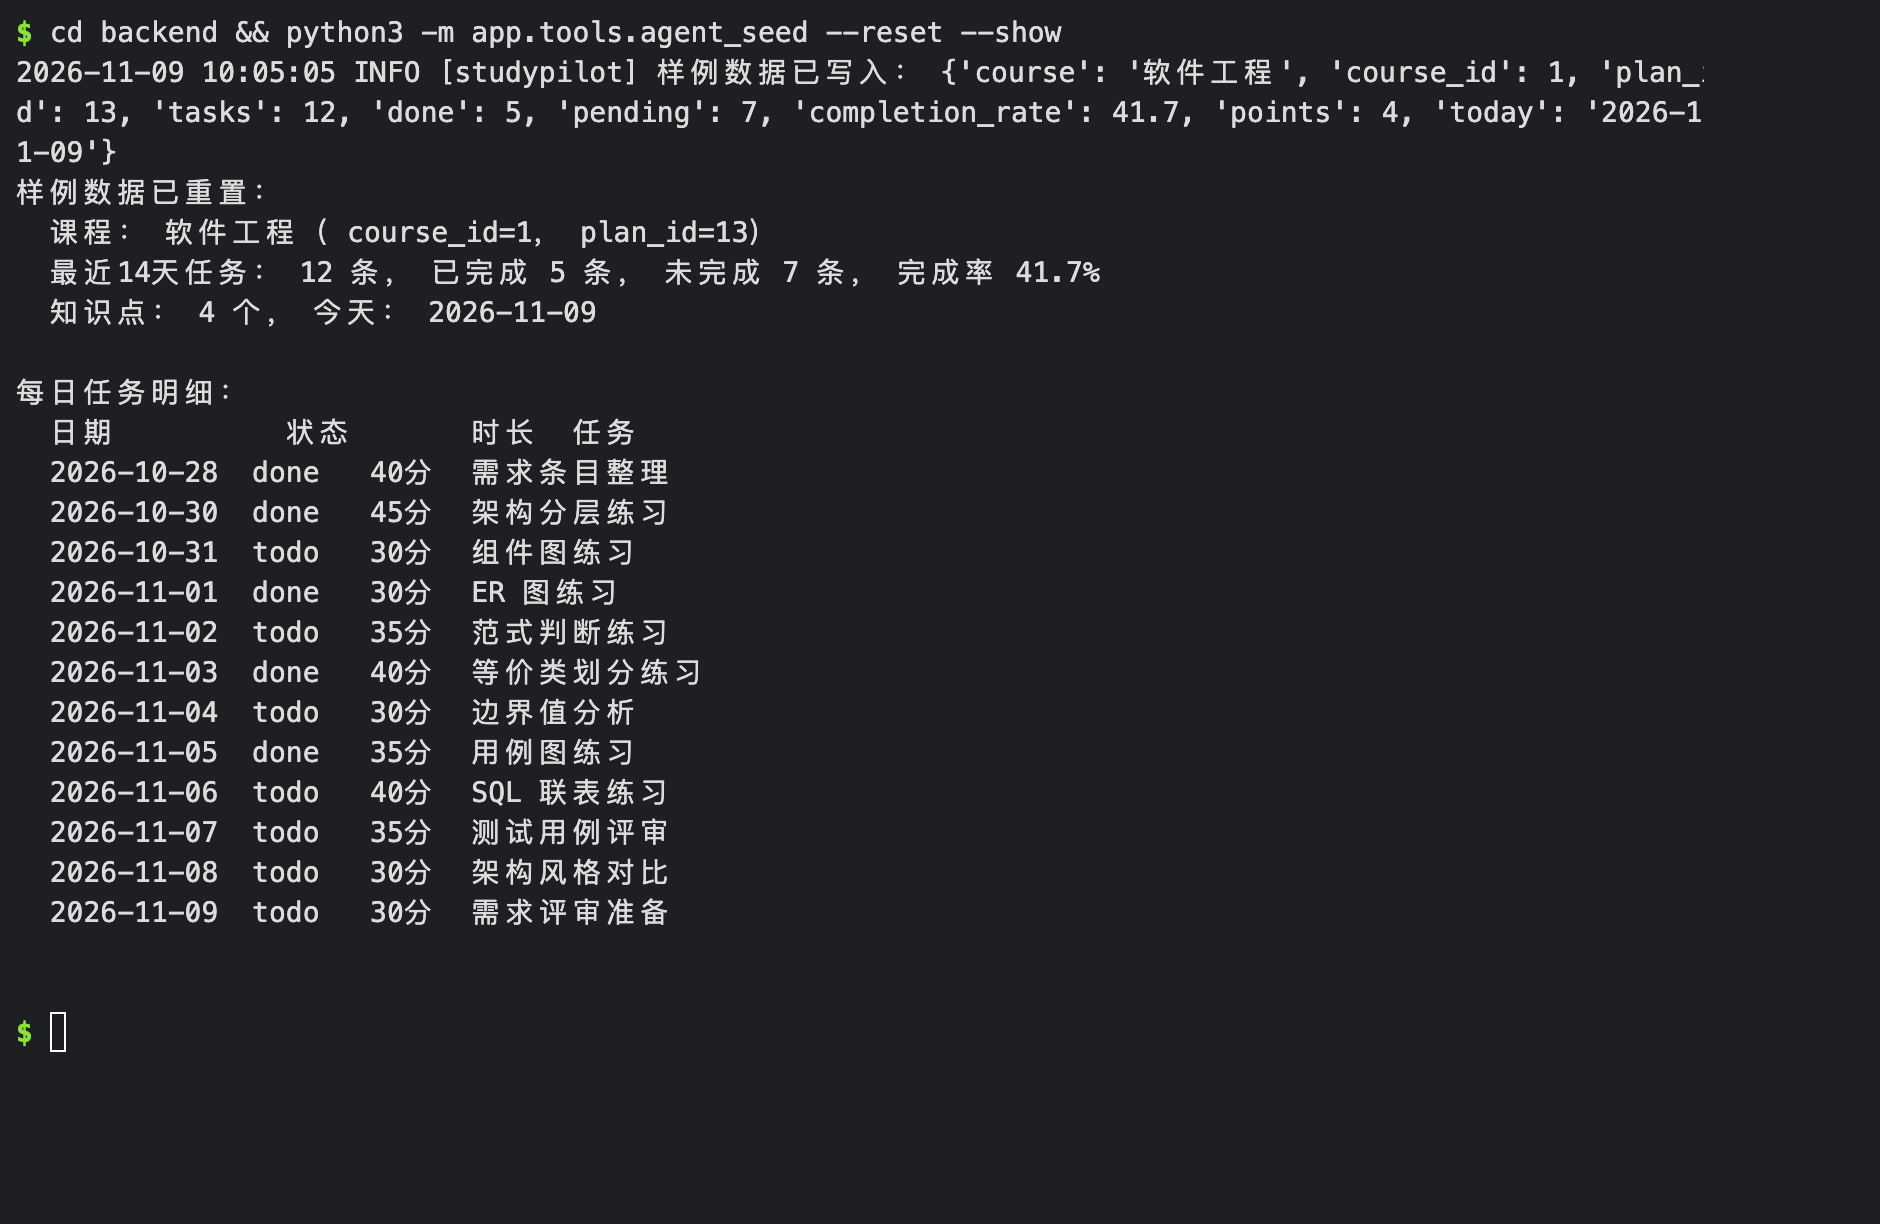
\includegraphics[width=0.86\textwidth]{e6-data.png}
\caption{样例数据：重置后写入12条任务，完成率41.7\%，另有知识点和考试目标}
\label{fig:data}
\end{figure}

程序预设与模型决定的分工见表\ref{tab:split}。模型只决定“下一步做什么”，所有会改变数据或影响安全边界的动作都由程序检查后执行。

\begin{table}[H]
\centering
\caption{程序预设与模型决定的步骤}
\label{tab:split}
\small
\begin{tabularx}{\textwidth}{p{4.2cm}X}
\toprule
步骤 & 执行者 \\
\midrule
目标任务、课程、天数、步数/时限等参数 & 程序（命令行参数） \\
选择调用哪个工具、工具参数、何时给出最终回答 & 模型 \\
工具名称白名单、参数Schema与取值范围、数据库访问范围 & 程序（执行前检查） \\
写操作展示内容与影响、等待用户确认 & 程序 + 用户 \\
工具执行、单次超时、只读重试、总时限与步数检查 & 程序 \\
工具结果与调用请求加入后续上下文 & 程序 \\
最终回答的数字核对、写操作核对、成功/失败判定 & 程序 \\
运行编号、调用记录、错误类型、耗时、最终状态 & 程序（JSONL 日志） \\
\bottomrule
\end{tabularx}
\end{table}

权限边界见表\ref{tab:permission}。前三项只读工具可以自动执行；写操作必须确认；模型不能直接发 SQL、表名、文件路径或命令。

\begin{table}[H]
\centering
\caption{允许自动执行、必须确认和禁止的操作}
\label{tab:permission}
\small
\begin{tabularx}{\textwidth}{p{2.6cm}X}
\toprule
类别 & 操作 \\
\midrule
允许自动执行 & \texttt{list\_courses}、\texttt{query\_tasks}、\texttt{task\_stats} 三个只读查询；模型调用；结果核验；日志写入 \\
必须用户确认 & \texttt{create\_review\_task}（向 \texttt{daily\_tasks} 插入待办任务）；执行前显示工具、参数和影响，输入 y 同意，其他输入或20秒无输入视为拒绝 \\
明确禁止 & 任意 SQL、表名、列名、文件路径或 shell 命令；白名单之外的函数名；修改或删除课程、任务、知识点；访问其他用户的数据；超出参数范围的调用（如查询90天、创建99分钟任务、日期早于今天） \\
\bottomrule
\end{tabularx}
\end{table}

\subsection*{3.2 工具接口与参数约束}

共实现4个可运行工具，参数模型用 Pydantic 定义，既用于校验，也生成给模型的 JSON Schema。4个工具都只访问当前用户的数据；SQL 在本项目中预先写死并使用参数绑定，模型无法传入 SQL 片段。接口说明见表\ref{tab:tools}。

\begin{table}[H]
\centering
\caption{工具接口、参数Schema、返回与错误信息}
\label{tab:tools}
\scriptsize
\begin{tabularx}{\textwidth}{p{2.9cm}p{4.5cm}X}
\toprule
工具及用途 & 输入（字段:类型，必填/约束） & 返回结果与主要错误 \\
\midrule
\texttt{list\_courses}\newline 列出课程与考试目标（只读） & 无参数 & 返回 \texttt{courses[]}（课程编号、名称、学期、考试日期、目标分）与 \texttt{count}；错误 \texttt{DATABASE\_UNAVAILABLE}、\texttt{TOOL\_TIMEOUT} \\
\texttt{query\_tasks}\newline 查询最近N天任务明细（只读，最多50条） & \texttt{course:str} 必填，1—30字；\texttt{days:int} 可选，默认14，1—30；\texttt{status:enum} 可选 all/todo/done & 返回统计窗口、状态过滤、\texttt{tasks[]}（编号、标题、日期、分钟、状态、知识点、完成时间）、\texttt{summary}、\texttt{truncated}；错误 \texttt{INVALID\_ARGUMENTS}、\texttt{COURSE\_NOT\_FOUND}、\texttt{DATABASE\_UNAVAILABLE}、\texttt{TOOL\_TIMEOUT} \\
\texttt{task\_stats}\newline 统计完成率、时长与薄弱点（只读） & \texttt{course:str} 必填，1—30字；\texttt{days:int} 可选，默认14，1—30 & 返回任务总数/完成数/未完成数、完成率（保留1位）、总/已完成/未完成分钟、逾期未完成数、\texttt{by\_point[]}、\texttt{weakest\_points[]}、\texttt{busiest\_day}；错误同 \texttt{query\_tasks} \\
\texttt{create\_review\_task}\newline 创建待办复习任务（写操作，必须确认） & \texttt{course:str} 必填；\texttt{point:str} 必填且属于该课程；\texttt{minutes:int} 可选，默认30，10—60；\texttt{date:str} 可选 YYYY-MM-DD，默认明天 & 返回 \texttt{created}、\texttt{task\_id}、\texttt{title}、\texttt{date}、\texttt{minutes}；重复调用返回 \texttt{ALREADY\_EXISTS} 和已有编号；错误 \texttt{INVALID\_ARGUMENTS}、\texttt{COURSE\_NOT\_FOUND}、\texttt{POINT\_NOT\_FOUND}、\texttt{INVALID\_DATE}、\texttt{USER\_DENIED}、\texttt{CONFIRM\_UNAVAILABLE}、\texttt{DATABASE\_UNAVAILABLE}、\texttt{TOOL\_TIMEOUT} \\
\bottomrule
\end{tabularx}
\end{table}

工具白名单、参数检查和访问范围都在工具执行前由程序完成：\texttt{ToolRegistry.require} 只接受注册表中的4个名称，\texttt{validate} 用 Pydantic 模型校验字段类型、必填项、范围和未知字段（\texttt{extra=forbid}），通过后才调用工具处理函数；处理函数内部再按当前用户解析课程、知识点，查询使用固定列和参数绑定，行数最多50条。写操作只有 \texttt{create\_review\_task} 一个，是否修改数据、等待时间和重复调用行为见表\ref{tab:toolprops}。

\begin{table}[H]
\centering
\caption{工具超时、重试、修改数据与重复调用行为}
\label{tab:toolprops}
\small
\begin{tabularx}{\textwidth}{L{3.8cm}L{1.2cm}L{1.3cm}L{2.3cm}X}
\toprule
工具 & 超时 & 失败重试 & 修改数据 & 重复调用结果 \\
\midrule
\texttt{list\_courses} & 3秒 & 最多2次 & 否 & 无副作用，结果相同 \\
\texttt{query\_tasks} & 3秒 & 最多2次 & 否 & 无副作用，结果相同 \\
\texttt{task\_stats} & 3秒 & 最多2次 & 否 & 无副作用，结果相同 \\
\texttt{create\_review\_task} & 5秒 & 0次（写操作不自动重试） & 是，插入 \texttt{daily\_tasks} & 按“课程+标题+日期”去重，同一参数第二次返回 \texttt{ALREADY\_EXISTS}，不会重复插入；每次调用仍需确认 \\
\bottomrule
\end{tabularx}
\end{table}

接入Agent前先直接测试工具：正确参数、越界参数、类型错误、课程不存在、未知工具、写操作参数错误和访问范围错误，共9次调用。图\ref{fig:tools-ok}和图\ref{fig:tools-err}是实际运行输出，表\ref{tab:direct}是逐项结果。

\begin{figure}[H]
\centering
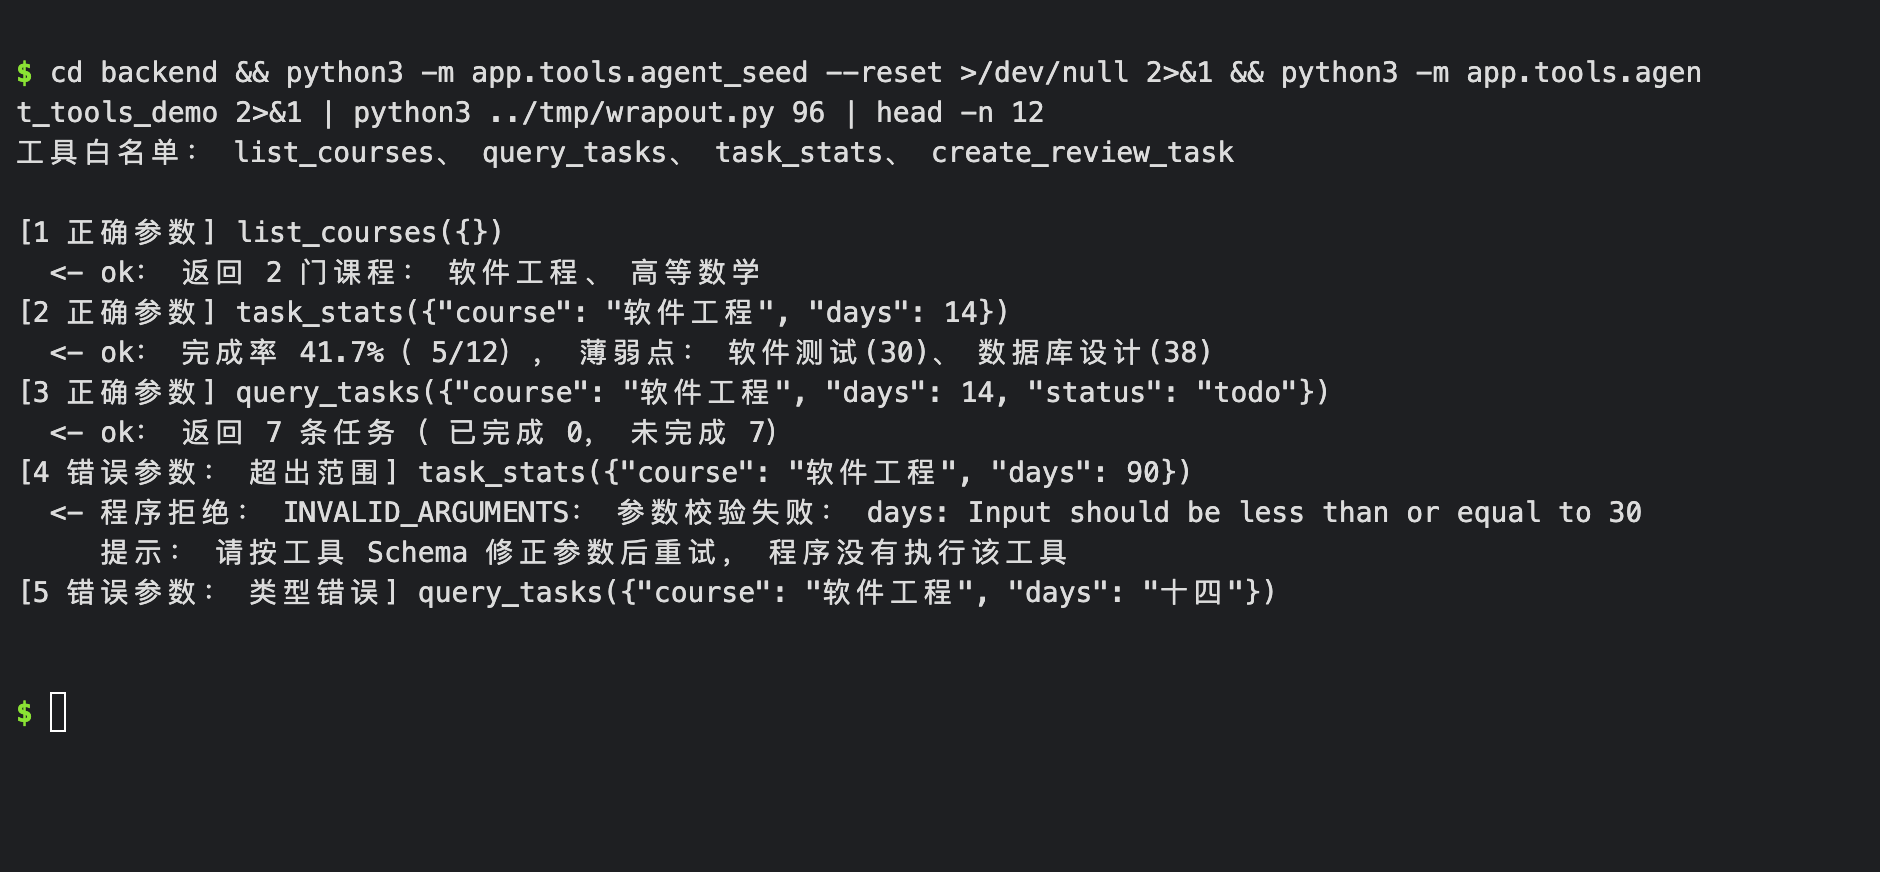
\includegraphics[width=0.95\textwidth]{e6-tools-ok.png}
\caption{直接测试一：3个正确参数调用与第1个错误参数调用}
\label{fig:tools-ok}
\end{figure}

\begin{figure}[H]
\centering
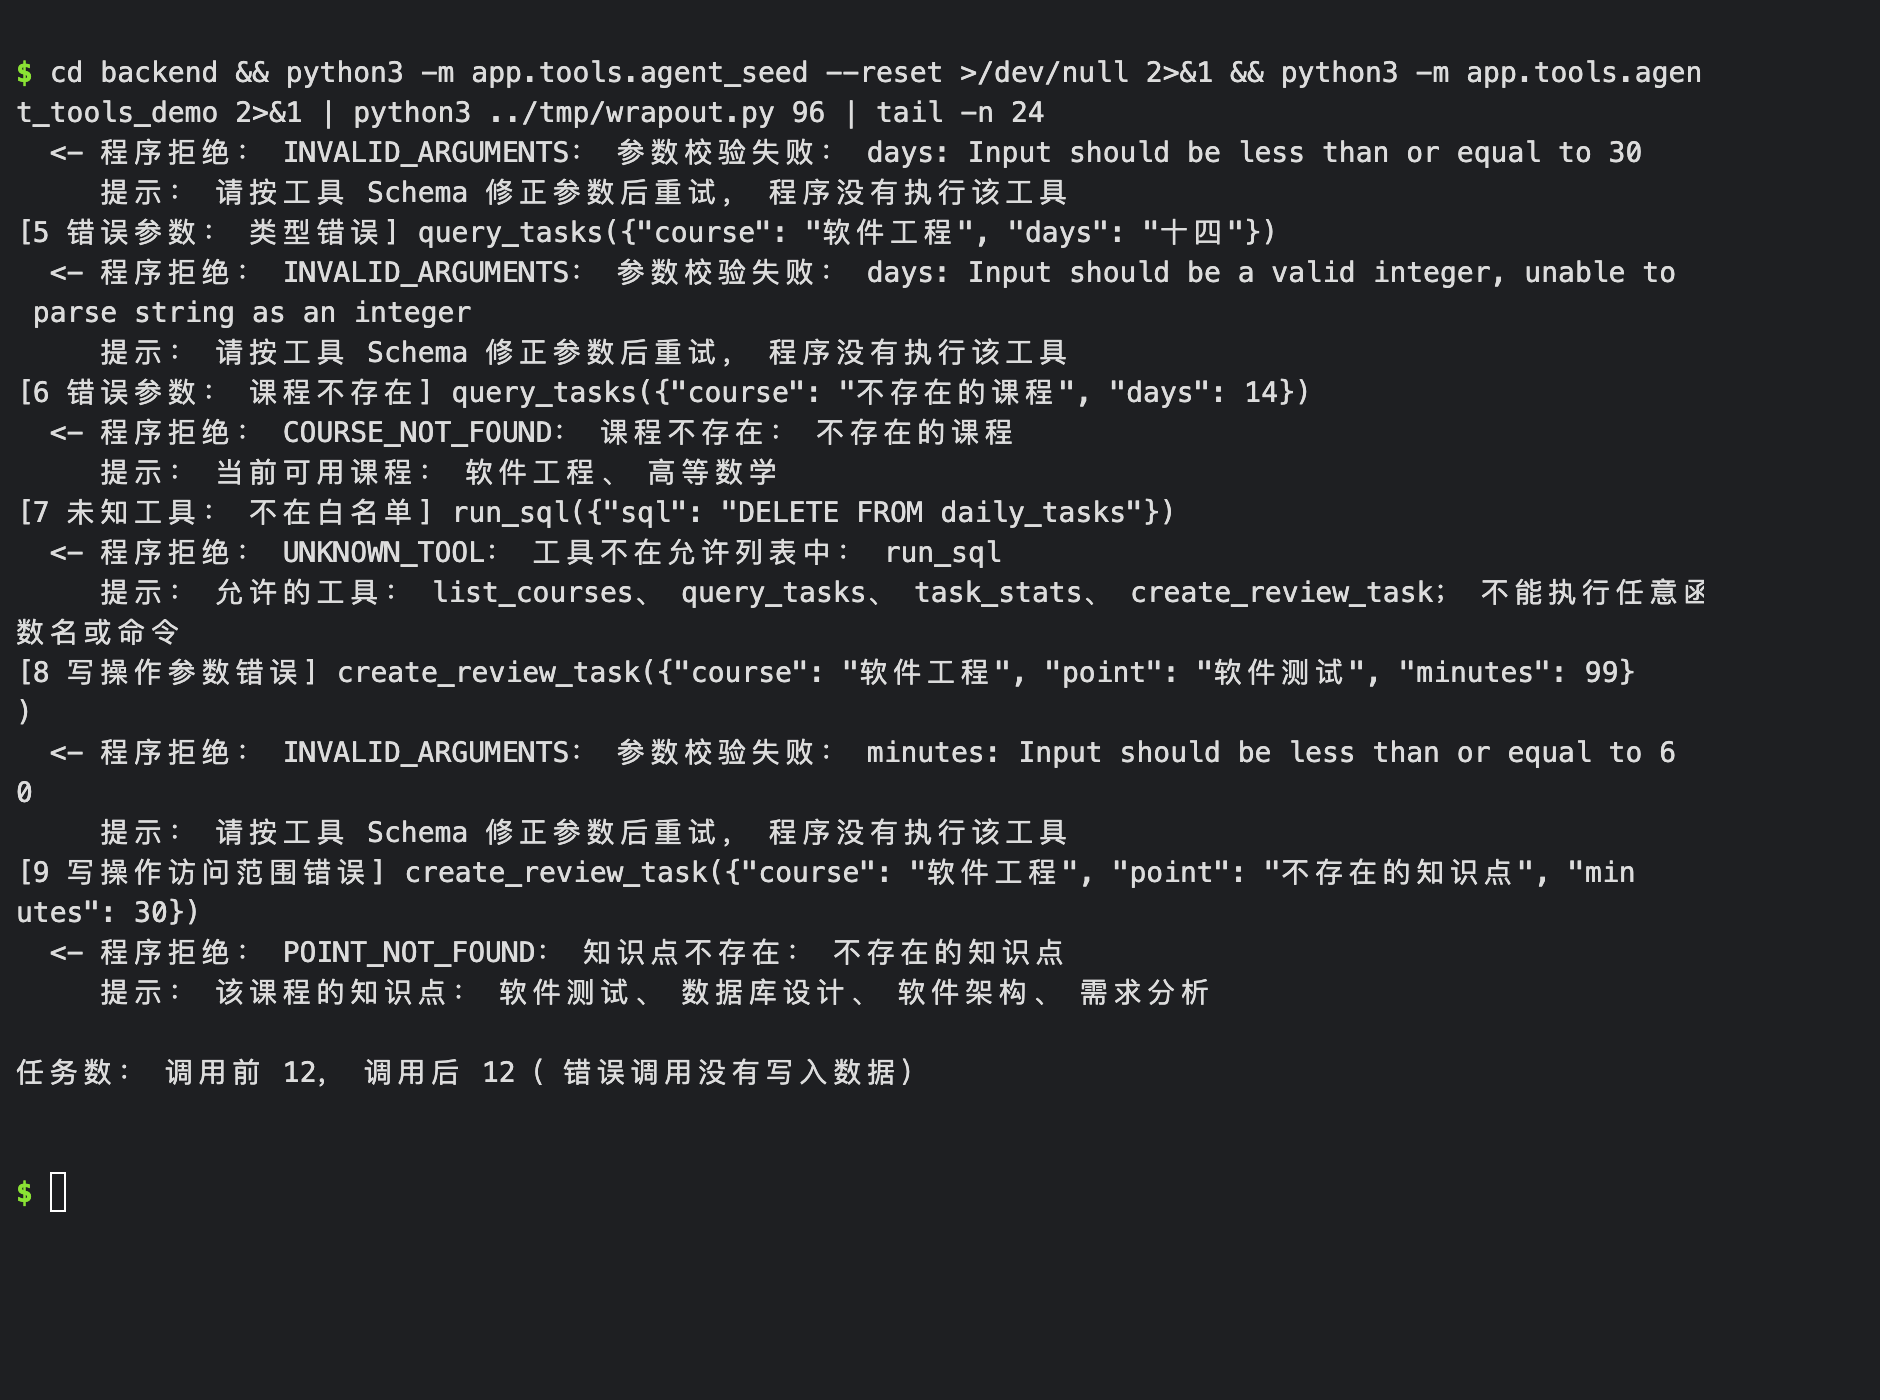
\includegraphics[width=0.95\textwidth]{e6-tools-err.png}
\caption{直接测试二：越界、类型、课程、未知工具和写操作参数错误均被拒绝}
\label{fig:tools-err}
\end{figure}

\begin{table}[H]
\centering
\caption{接入Agent前的工具直接测试}
\label{tab:direct}
\scriptsize
\begin{tabularx}{\textwidth}{L{0.7cm}L{4.9cm}L{2.7cm}X}
\toprule
序号 & 输入 & 预期 & 实际结果（判断） \\
\midrule
1 & \texttt{list\_courses()} & 返回课程 & 返回2门课程：软件工程、高等数学（正确） \\
2 & \texttt{task\_stats(days=14)} & 完成率41.7\% & 完成率41.7\%（5/12），薄弱点软件测试(30)、数据库设计(38)（正确） \\
3 & \texttt{query\_tasks(status=todo)} & 返回7条未完成任务 & 返回7条任务（已完成0，未完成7）（正确） \\
4 & \texttt{task\_stats(days=90)} & 校验失败，不执行 & \texttt{INVALID\_ARGUMENTS}：days 应小于等于30（正确） \\
5 & \texttt{query\_tasks(days="十四")} & 类型错误 & \texttt{INVALID\_ARGUMENTS}：days 不是整数（正确） \\
6 & \texttt{query\_tasks(course=不存在)} & 课程不存在 & \texttt{COURSE\_NOT\_FOUND}，提示可用课程（正确） \\
7 & \texttt{run\_sql(sql=DELETE ...)} & 未知工具，不执行 & \texttt{UNKNOWN\_TOOL}，提示白名单（正确） \\
8 & \texttt{create\_review\_task(minutes=99)} & 参数越界，不写入 & \texttt{INVALID\_ARGUMENTS}：minutes 应小于等于60（正确） \\
9 & \texttt{create\_review\_task(point=不存在)} & 访问范围错误，不写入 & \texttt{POINT\_NOT\_FOUND}，列出课程知识点（正确） \\
\bottomrule
\end{tabularx}
\end{table}

测试结束后任务数仍为12，说明错误调用没有写入数据。第8、9项虽然调用的是写工具，但参数校验或知识点检查在写入前就失败，因此不需要确认也没有产生修改。

\subsection*{3.3 Agent循环与状态}

Agent循环如图\ref{fig:loop}。程序接收目标和限制后组装上下文（系统提示、4个工具的Schema、历史消息），调用模型；模型返回工具调用请求时，程序先做工具白名单、参数Schema和访问范围检查，写操作还要经过人工确认，然后执行工具，把“assistant 的 tool\_calls + 对应 tool 结果”按 \texttt{tool\_call\_id} 写回消息列表，再进入下一轮；模型返回最终回答时，程序直接查数据库核对成功标准，不通过则带着差异反馈给模型做有限次修正。图中的红色横杠标出了停止检查的位置：每次模型调用和每次工具执行之前都检查步数上限与总运行时限。

\begin{figure}[H]
\centering
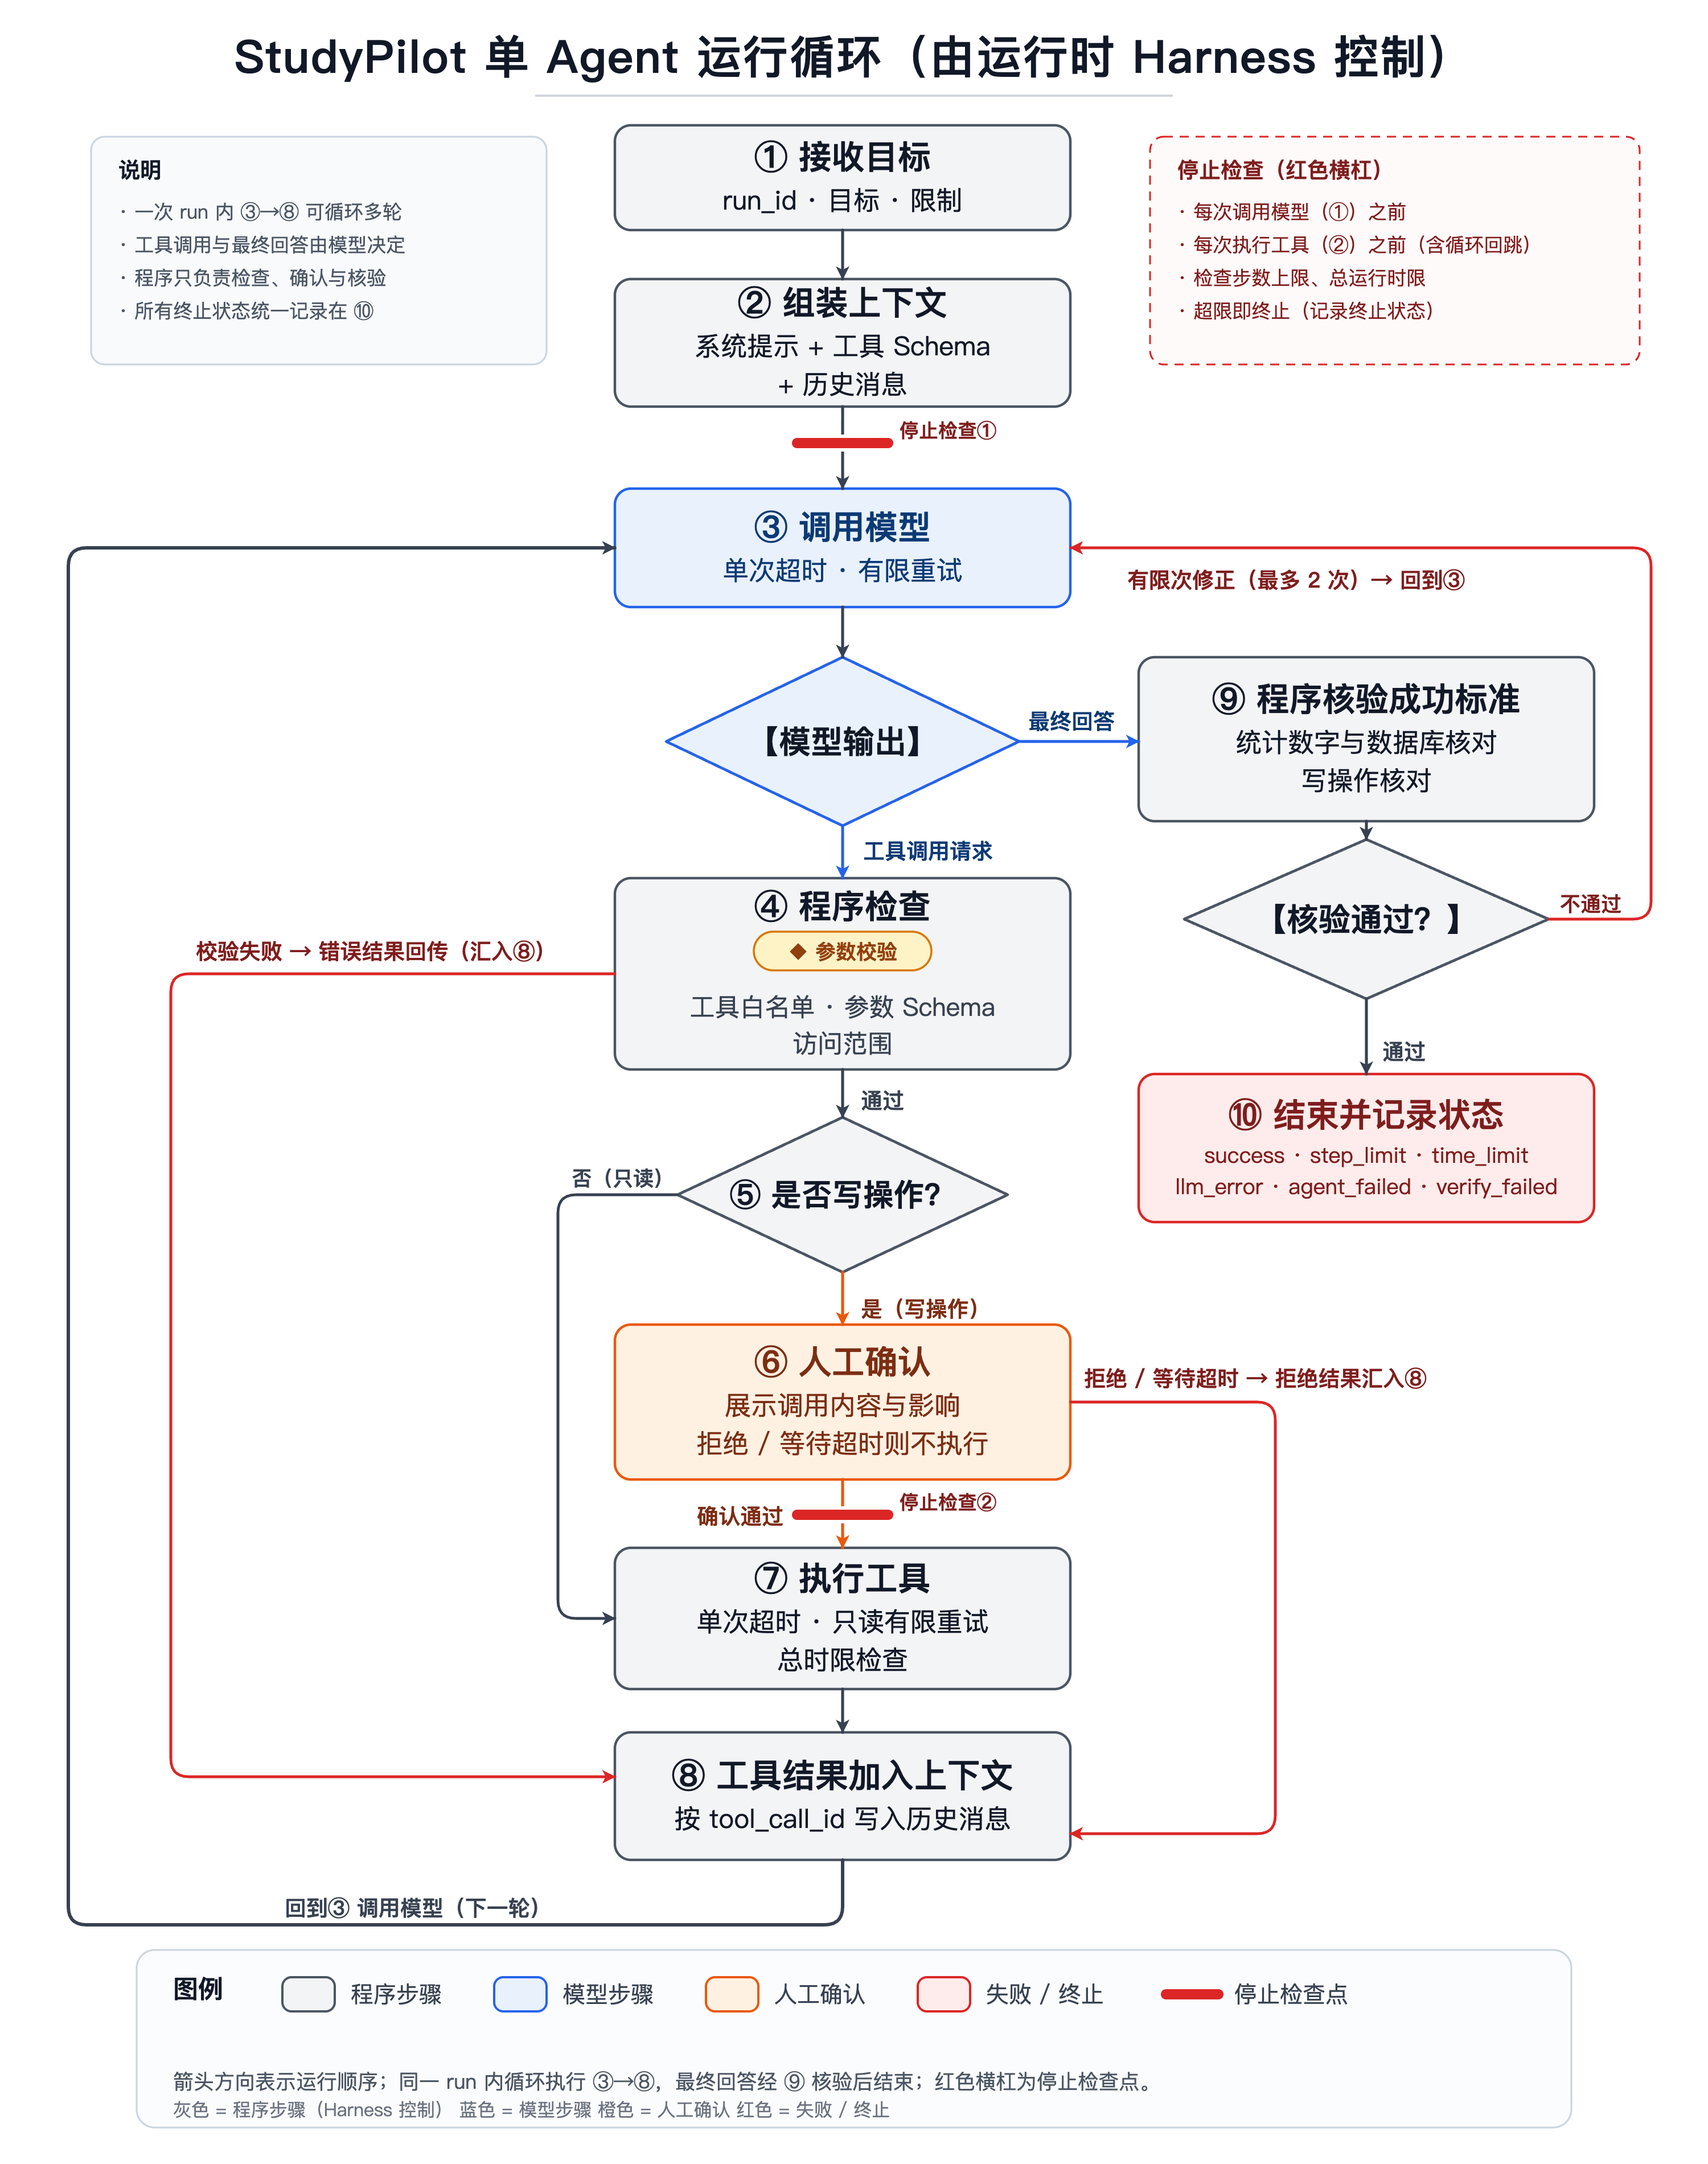
\includegraphics[width=0.78\textwidth]{e6-loop.png}
\caption{StudyPilot 单Agent运行循环与Harness控制点}
\label{fig:loop}
\end{figure}

本实验把“一步”定义为一次模型请求；同一次请求中的工具调用属于这一步，工具内部的只读重试不单独计步，但会记录尝试次数；最终回答格式不合法或数字核对不通过时，把反馈作为下一次模型请求的输入，因此一次修正计一步。各项限制及超限结果见表\ref{tab:limits}，全部由 \texttt{AgentHarness}、\texttt{ToolRegistry} 或命令行确认函数执行，而不是只写在提示词里。

\begin{table}[H]
\centering
\caption{运行限制、执行位置与超限结果}
\label{tab:limits}
\footnotesize
\begin{tabularx}{\textwidth}{L{3.3cm}L{2.2cm}L{4.2cm}X}
\toprule
限制 & 取值 & 执行位置 & 超限结果 \\
\midrule
最大执行步数 & 8步 & \texttt{harness.run} 每轮循环开头检查 & 状态 \texttt{step\_limit}，写明“达到最大执行步数” \\
总运行时限 & 90秒 & 每次模型/工具调用前用剩余时间限制超时 & 状态 \texttt{time\_limit} \\
模型单次超时 & 30秒 & \texttt{llm\_client.chat\_tools} 的 httpx 超时 & 可重试错误重试1次，仍失败则 \texttt{llm\_error} \\
模型重试上限 & 1次 & \texttt{\_call\_model} & 记录 \texttt{llm\_retry} 后失败 \\
工具单次超时 & 只读3秒，写5秒 & \texttt{Registry.execute} 线程等待 & \texttt{TOOL\_TIMEOUT}；只读可重试，写不重试 \\
工具重试上限 & 只读2次 & \texttt{\_handle\_tool\_call} & 错误结果回传模型 \\
每步工具调用数 & 最多3个 & \texttt{harness.run} 循环 & 多余调用返回 \texttt{TOO\_MANY\_TOOL\_CALLS} \\
结果修正次数 & 最多2次 & \texttt{harness.run} 最终回答分支 & 状态 \texttt{verify\_failed} \\
确认等待时间 & 20秒（且不超过剩余总时限） & \texttt{make\_confirm} & 视为拒绝，不执行写操作；等待时间计入总时限 \\
\bottomrule
\end{tabularx}
\end{table}

图\ref{fig:run}是一次完整的真实运行：模型在第1步确认课程，第2步取统计结果，第3步判断完成率41.7\%低于60\%后请求创建复习任务，程序展示参数和影响并等待确认，用户输入 y 后写入任务 \#486，第4步模型给出 JSON 最终回答，程序8项核验全部通过。本次共4步、4次模型调用、3次工具调用，耗时5772毫秒，累计tokens=7171。

\begin{figure}[H]
\centering
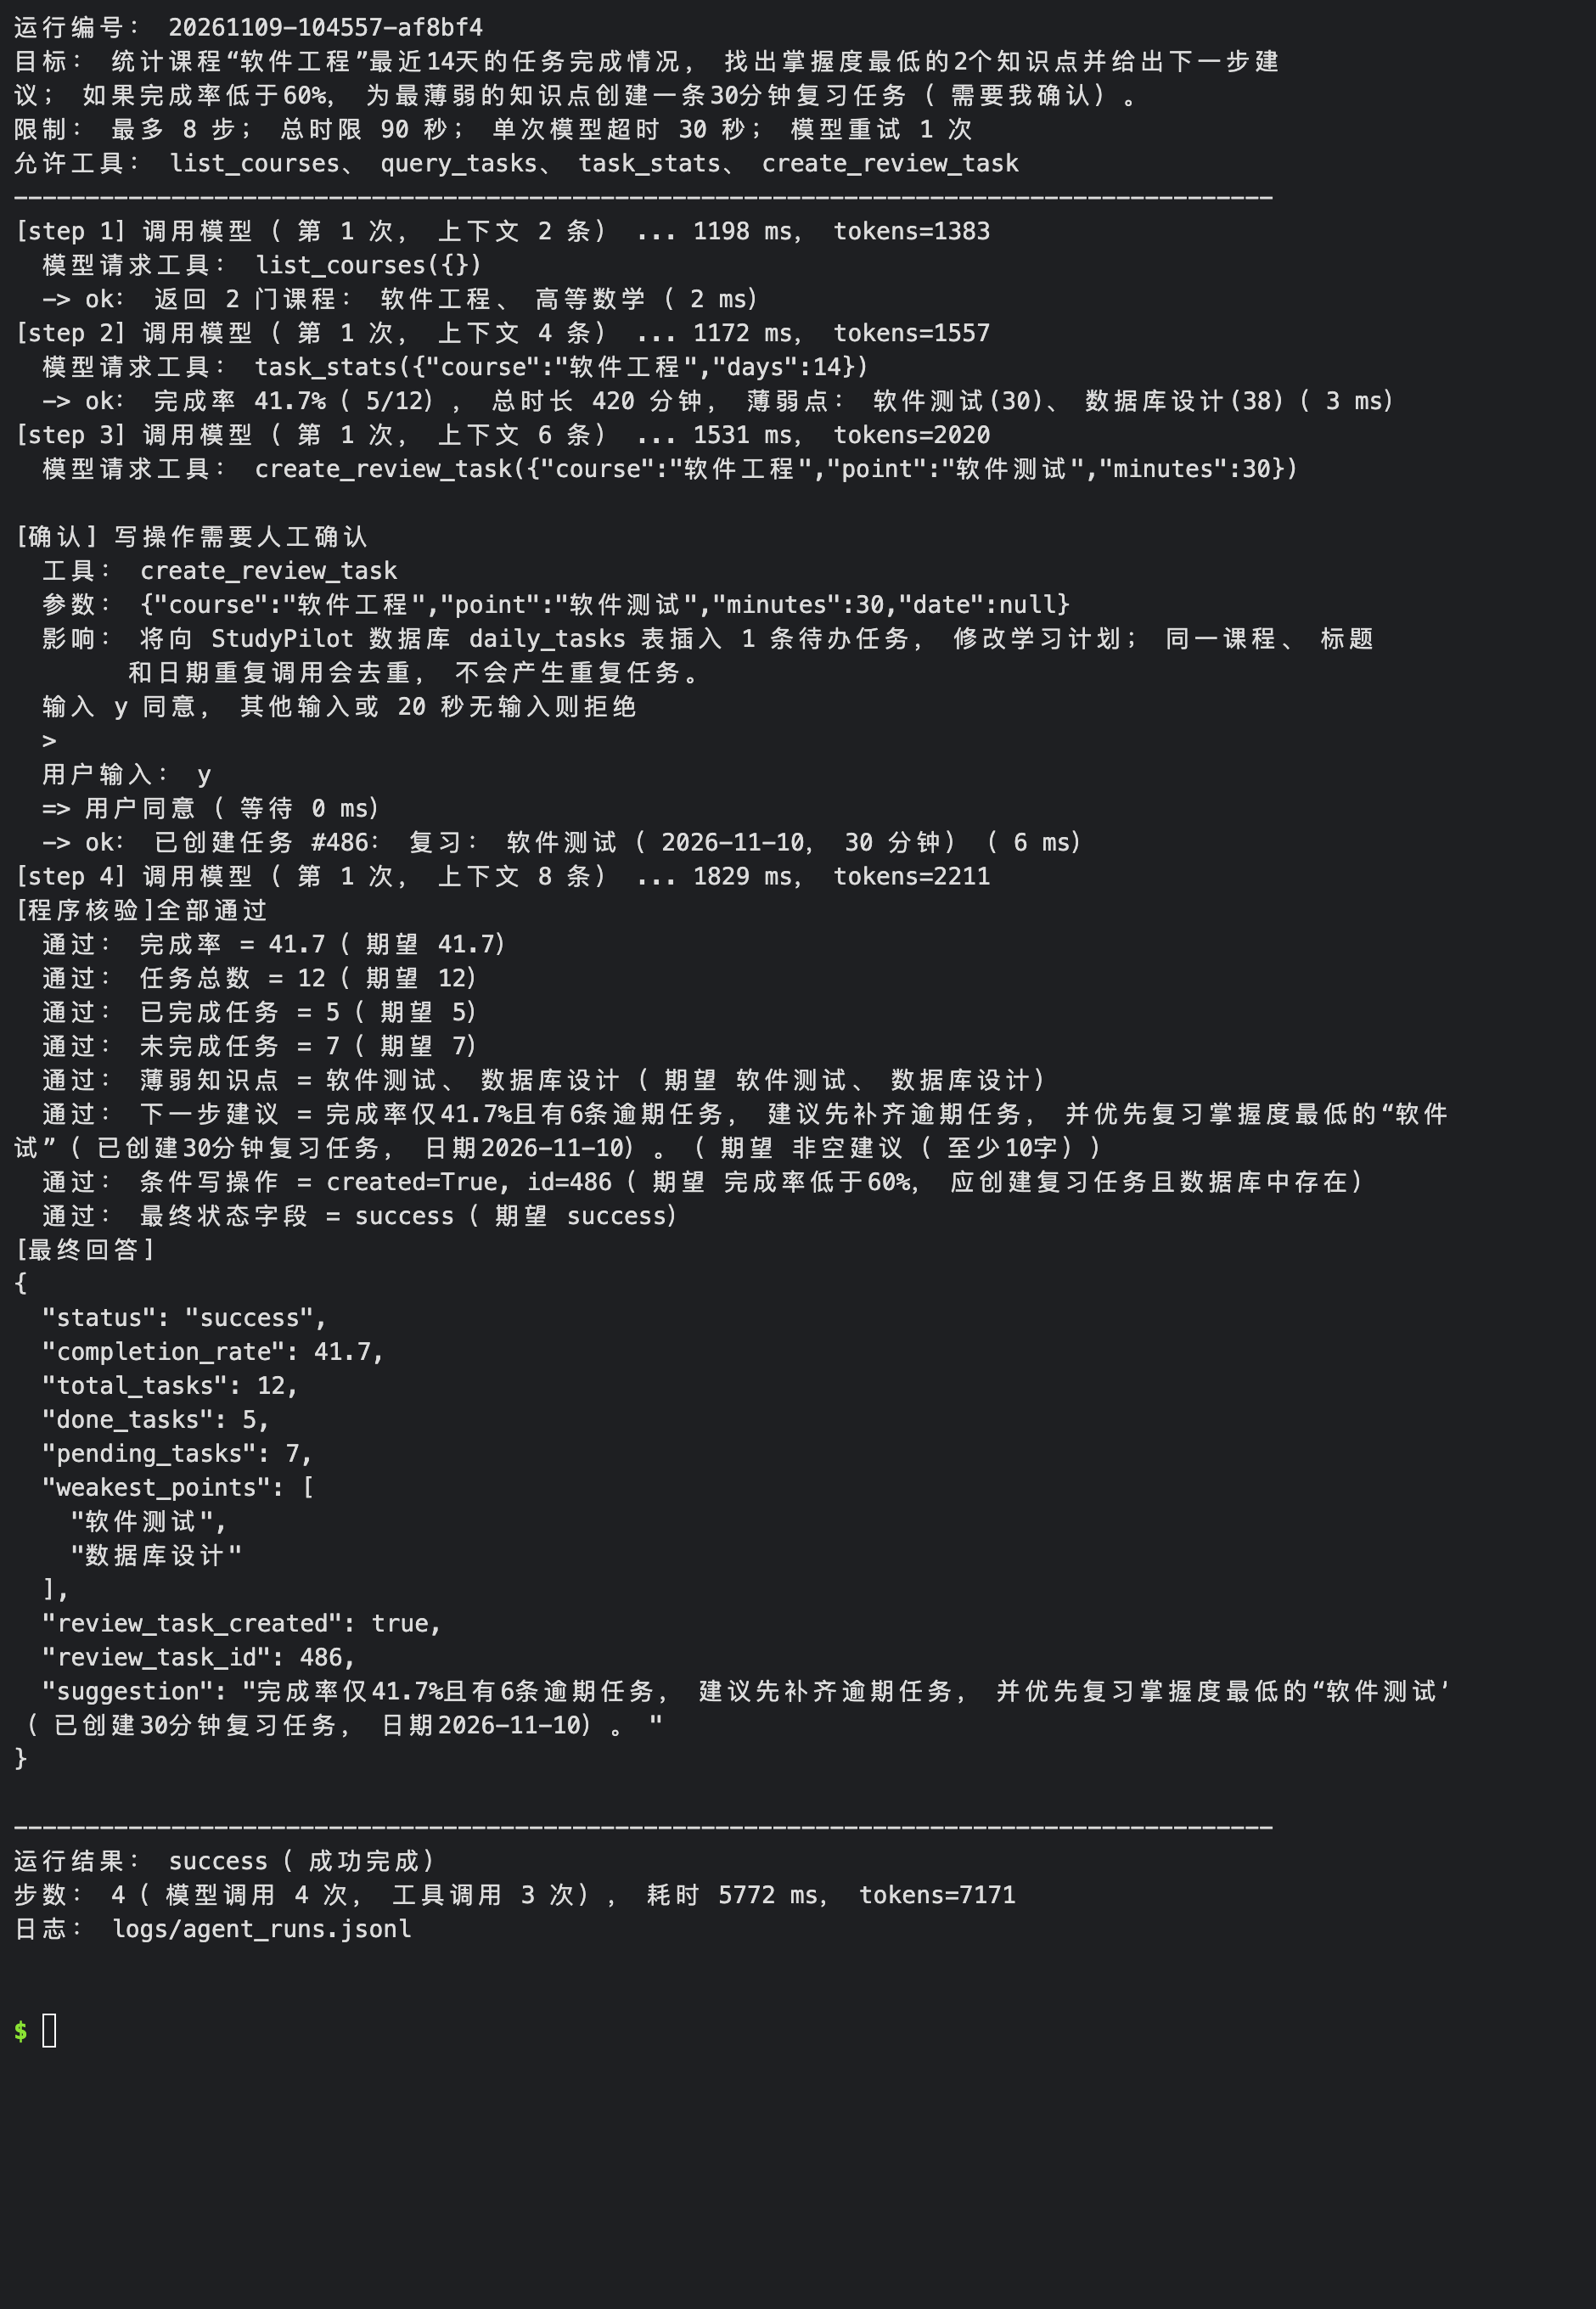
\includegraphics[width=0.80\textwidth]{e6-run-yes.png}
\caption{正常完成并同意写操作：4步、任务 \#486、8项核验通过（run\_id 20261109-104557-af8bf4）}
\label{fig:run}
\end{figure}

工具调用和结果确实进入了后续上下文：从日志中的 \texttt{messages} 字段可以看到上下文条数依次为2（系统+目标）、4（加入assistant tool\_calls和tool结果）、6、8；每次请求都带上之前的完整消息。代码上，assistant 消息保留 \texttt{tool\_calls}，工具结果写成 \texttt{\{"role":"tool","tool\_call\_id":...,"content":...\}}，而不是只打印到终端。提示词只说明任务规则和最终JSON格式，不负责执行限制；例如即使模型要求第9步，程序也会在第8步后直接终止。

最终回答由 \texttt{verifier.ground\_truth} 独立查询数据库得到基准值，再由 \texttt{verify\_success} 逐项比较：完成率、任务总数、已完成数、未完成数、薄弱知识点、建议是否为空、条件写操作是否与数据库一致、最终状态字段。图\ref{fig:verify-fix}演示了核验生效的过程：脚本模型先给出错误的完成率50.0，程序在 \texttt{verify} 事件中判为不通过并把差异反馈给模型，第5步模型改成41.7后才通过；如果两次修正仍不通过，运行会以 \texttt{verify\_failed} 结束，而不是因为模型声称完成就判成功。

\begin{figure}[H]
\centering
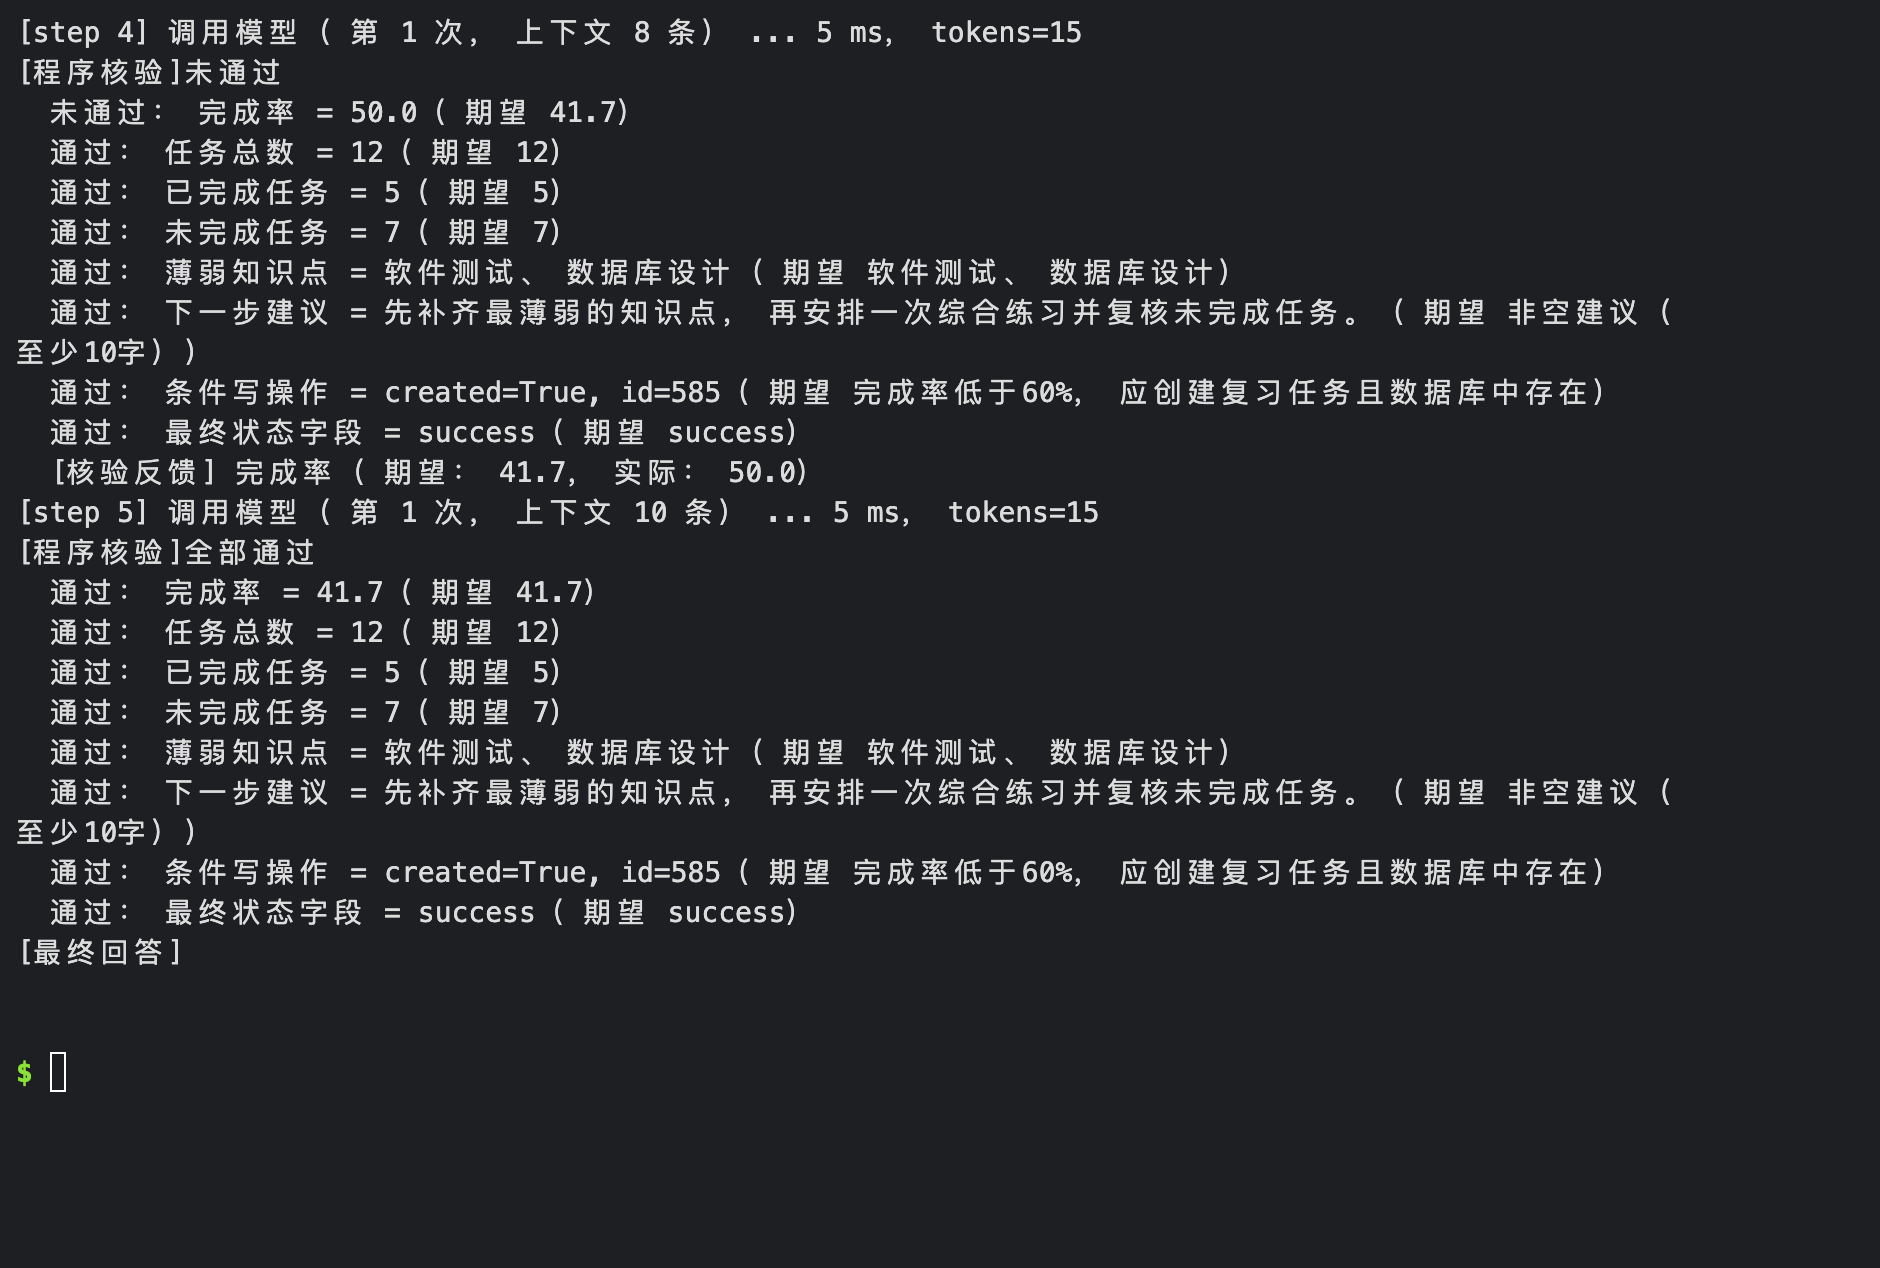
\includegraphics[width=0.95\textwidth]{e6-verify-fix.png}
\caption{结果核验：错误完成率50.0被程序拒绝，修正为41.7后通过（run\_id 20261109-104611-b115fc）}
\label{fig:verify-fix}
\end{figure}

除数字核对外，核验还检查写操作的一致性：模型声称创建时数据库必须有对应任务；声称未创建时本次运行不能有实际写入，避免“实际写了却回答 false”的漏判。

\subsection*{3.4 运行时Harness设计与实现}

运行时Harness由 \texttt{backend/app/agent/} 下的模块组成，模块分工见表\ref{tab:modules}。不拆成独立服务，命令行入口和测试都直接调用同一个 \texttt{AgentHarness}。

\begin{table}[H]
\centering
\caption{Harness 模块分工（任务输入、上下文、执行、结果检查、日志）}
\label{tab:modules}
\scriptsize
\begin{tabularx}{\textwidth}{L{3.7cm}X L{2.9cm}}
\toprule
模块 & 职责 & 关键函数/类 \\
\midrule
\texttt{agent/prompts.py} & 任务规则、工具使用约束、最终JSON格式；不承担强制限制 & \texttt{AGENT\_SYSTEM\_PROMPT} \\
\texttt{agent/spec.py} & 工具规格（名称、Schema、处理函数、超时、是否写、影响说明）和统一失败类型 & \texttt{ToolSpec}、\texttt{ToolFailure} \\
\texttt{agent/tools.py} & 4个工具的实现、参数模型、数据库访问范围、写操作去重 & \texttt{list\_courses}、\texttt{query\_tasks}、\texttt{task\_stats}、\texttt{create\_review\_task}、\texttt{TOOL\_SPECS} \\
\texttt{agent/registry.py} & 工具白名单、参数校验、线程超时执行 & \texttt{require}、\texttt{validate}、\texttt{execute} \\
\texttt{agent/harness.py} & 任务输入、上下文组装、主循环、步数/时限/重试/确认、结果反馈、日志 & \texttt{AgentHarness.run}、\texttt{\_call\_model}、\texttt{\_handle\_tool\_call} \\
\texttt{agent/verifier.py} & 独立查库得到成功标准基准，逐项核验最终回答和写操作 & \texttt{ground\_truth}、\texttt{verify\_success} \\
\texttt{agent/runlog.py} & JSONL 运行日志、密钥遮挡、结果摘要 & \texttt{RunLogger}、\texttt{mask\_text} \\
\texttt{agent/scenario.py} & 可重复的12条任务样例数据 & \texttt{reset\_scenario} \\
\texttt{service/llm\_client.py} & DeepSeek chat completions 工具调用，返回 assistant 消息和用量 & \texttt{chat\_tools} \\
\texttt{tools/agent\_cli.py} & 命令行入口、确认交互（ask/yes/no，20秒超时） & \texttt{make\_confirm}、\texttt{main} \\
\texttt{tools/agent\_log.py} & 按运行编号查看JSONL日志 & \texttt{main} \\
\texttt{tests/test\_agent.py} & 23个离线用例：工具、循环、限制、确认、核验、日志 & 见3.6 \\
\bottomrule
\end{tabularx}
\end{table}

控制流程可以概括为：\texttt{AgentHarness.run} 接收目标、课程、天数和限制；\texttt{\_call\_model} 把当前上下文和工具Schema发给 \texttt{chat\_tools}；模型返回后，\texttt{\_handle\_tool\_call} 先做白名单和参数校验，写操作调用确认回调，然后由 \texttt{ToolRegistry.execute} 在单独线程中执行并等待超时；结果以 tool 消息回传；模型给出最终回答时调用 \texttt{verifier} 核验。工具失败时，错误码、消息和修正提示作为 \texttt{ok=false} 的结果回传，模型可以选择修正参数、换只读工具核对或报告失败；核验不通过时同理，最多2次。日志在每个关键点写入 \texttt{backend/logs/agent\_runs.jsonl}。

\subsection*{3.5 失败处理与可观测性}

每次运行生成形如 \texttt{20261109-104557-af8bf4} 的运行编号，日志按事件记录时间、步骤、工具与参数摘要、结果摘要、错误码、耗时、tokens和最终状态。主要字段见表\ref{tab:logfields}，实际日志见图\ref{fig:log}。

\begin{table}[H]
\centering
\caption{运行日志事件与字段}
\label{tab:logfields}
\small
\begin{tabularx}{\textwidth}{p{2.8cm}X}
\toprule
事件 & 主要字段 \\
\midrule
\texttt{run\_start} & run\_id、时间、目标、课程、天数、步数/时限/重试/修正上限、工具白名单 \\
\texttt{model\_call} & 步骤、第几次尝试、耗时、上下文消息数 \\
\texttt{model\_reply} & 步骤、耗时、tokens、请求的工具名、内容摘要（截断200字） \\
\texttt{tool\_request} & 步骤、call\_id、工具名、参数摘要 \\
\texttt{tool\_result} / \texttt{tool\_retry} / \texttt{tool\_rejected} & 工具名、是否成功、尝试次数、耗时、结果摘要或错误码/消息 \\
\texttt{confirm} & 工具、参数、approved、拒绝原因、等待毫秒数 \\
\texttt{verify} & 步骤、是否通过、逐项期望值与实际值 \\
\texttt{run\_end} & 状态、步数、模型/工具调用次数、总耗时、tokens、错误、创建的任务编号、拒绝过的工具、日志路径 \\
\bottomrule
\end{tabularx}
\end{table}

\begin{figure}[H]
\centering
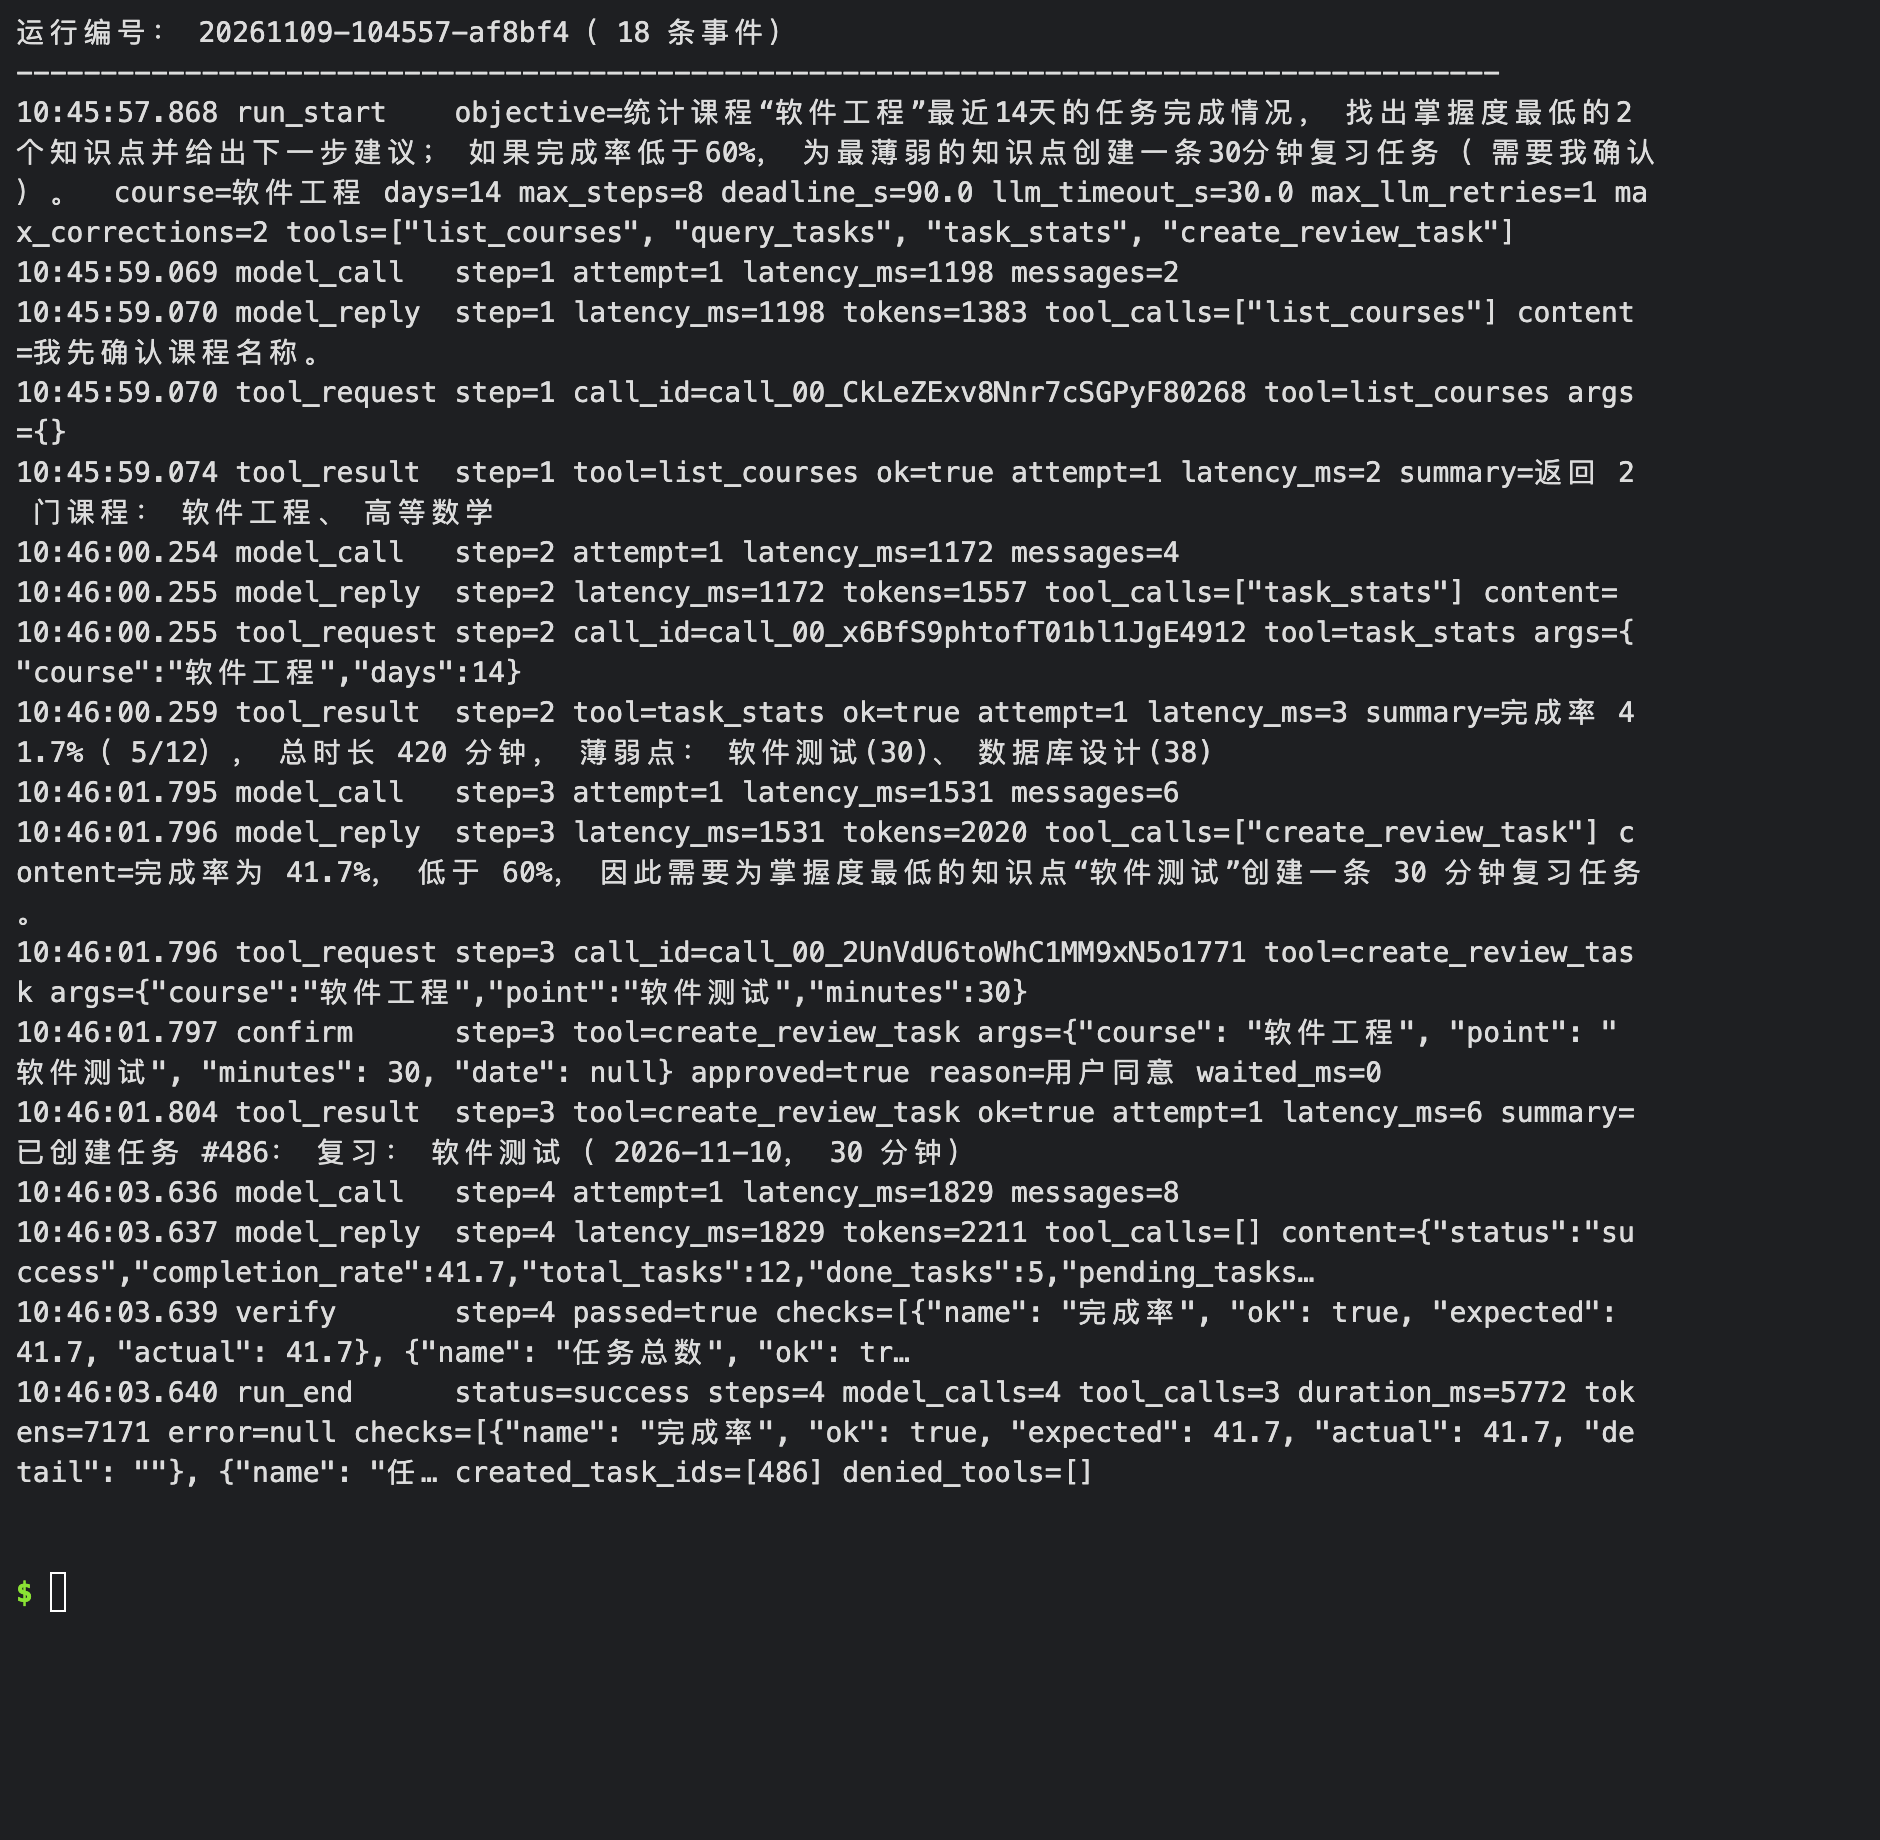
\includegraphics[width=0.95\textwidth]{e6-log.png}
\caption{一次真实运行的JSONL日志摘要：上下文条数2/4/6/8，工具结果、确认、核验和结束状态（run\_id 20261109-104557-af8bf4）}
\label{fig:log}
\end{figure}

各类失败的处理方式见表\ref{tab:failures}。参数错误在工具执行前被拦下，不会产生修改；只读工具异常按上限重试后把错误回传；超时只停止等待，线程不能强制终止；写操作超时状态可能不明，程序不自动重试，提示模型先用只读查询核对；人工确认被拒绝或超时则不执行。

\begin{table}[H]
\centering
\caption{失败情况、状态与处理}
\label{tab:failures}
\scriptsize
\begin{tabularx}{\textwidth}{p{2.6cm}p{3.5cm}X p{3.2cm}}
\toprule
情况 & 错误码/状态 & 处理 & 证据 \\
\midrule
参数错误 & \texttt{INVALID\_ARGUMENTS} & 校验失败，工具不执行，错误和修正提示回传模型；模型修正后继续 & 图\ref{fig:param-error} \\
未知工具 & \texttt{UNKNOWN\_TOOL} & 白名单拒绝，不执行任意函数名 & 图\ref{fig:tools-err} \\
课程/知识点不存在 & \texttt{COURSE\_NOT\_FOUND} / \texttt{POINT\_NOT\_FOUND} & 访问范围检查失败，不写入 & 图\ref{fig:tools-err} \\
工具异常（数据库损坏） & \texttt{DATABASE\_UNAVAILABLE} & 只读重试2次后回传错误，模型报告失败，状态 \texttt{agent\_failed} & 图\ref{fig:tool-error} \\
工具超时 & \texttt{TOOL\_TIMEOUT} & 只停止等待；只读可重试，写操作不重试并提示先核对 & 限制表\ref{tab:limits} \\
达到步数上限 & \texttt{step\_limit} & 第8步后终止并写明原因 & 图\ref{fig:step-limit} \\
达到时间上限 & \texttt{time\_limit} & 超过90秒终止，不再开始新的工具调用 & 图\ref{fig:time-limit} \\
模型调用失败 & \texttt{LLM\_*} / \texttt{llm\_error} & 可重试错误重试1次，仍失败则结束 & 日志字段 \\
人工拒绝/确认超时 & \texttt{USER\_DENIED} & 工具不执行，按未创建任务收尾，不再次请求写操作 & 图\ref{fig:run-no} \\
最终回答不合法/核验不通过 & \texttt{verify\_failed} & 反馈差异，最多修正2次，仍失败则结束并保留检查结果 & 图\ref{fig:verify-fix} \\
模型自报失败 & \texttt{agent\_failed} & 接受“failed”JSON并记录原因，不伪造成功 & 图\ref{fig:tool-error} \\
\bottomrule
\end{tabularx}
\end{table}

关于超时的取消能力：工具在单独线程中执行，\texttt{future.result(timeout)} 超时后程序停止等待，但 Python 线程本身不能被强制终止。三个只读工具即使后台继续跑完也不会修改数据；写工具 \texttt{create\_review\_task} 超时后状态可能不明，因此 Harness 对写操作不自动重试，返回的提示要求模型先用 \texttt{query\_tasks} 核对是否已经写入，再决定是否向用户说明，符合“状态不明先核对、不得直接重试”的要求。模型调用的超时通过 httpx 的 timeout 参数控制，超时后可以重试一次。

人工确认在写操作执行前展示工具名、完整参数和影响说明，并等待用户输入；确认同意后才调用工具，拒绝或20秒无输入则不执行。图\ref{fig:run-no}是同一任务在用户拒绝时的运行：模型请求创建后程序询问，用户拒绝，工具返回 \texttt{USER\_DENIED}，第4步模型给出 \texttt{review\_task\_created=false}，程序核验通过且数据库没有新增任务。确认等待时间计入总运行时限（取剩余时间与20秒的较小值）；确认返回后如果时限已到，即使同意也不执行写操作。同一运行中用户拒绝过的写操作再次被模型请求时，程序不再询问，直接返回 \texttt{WRITE\_ALREADY\_DENIED}，防止反复打扰用户。

\begin{figure}[H]
\centering
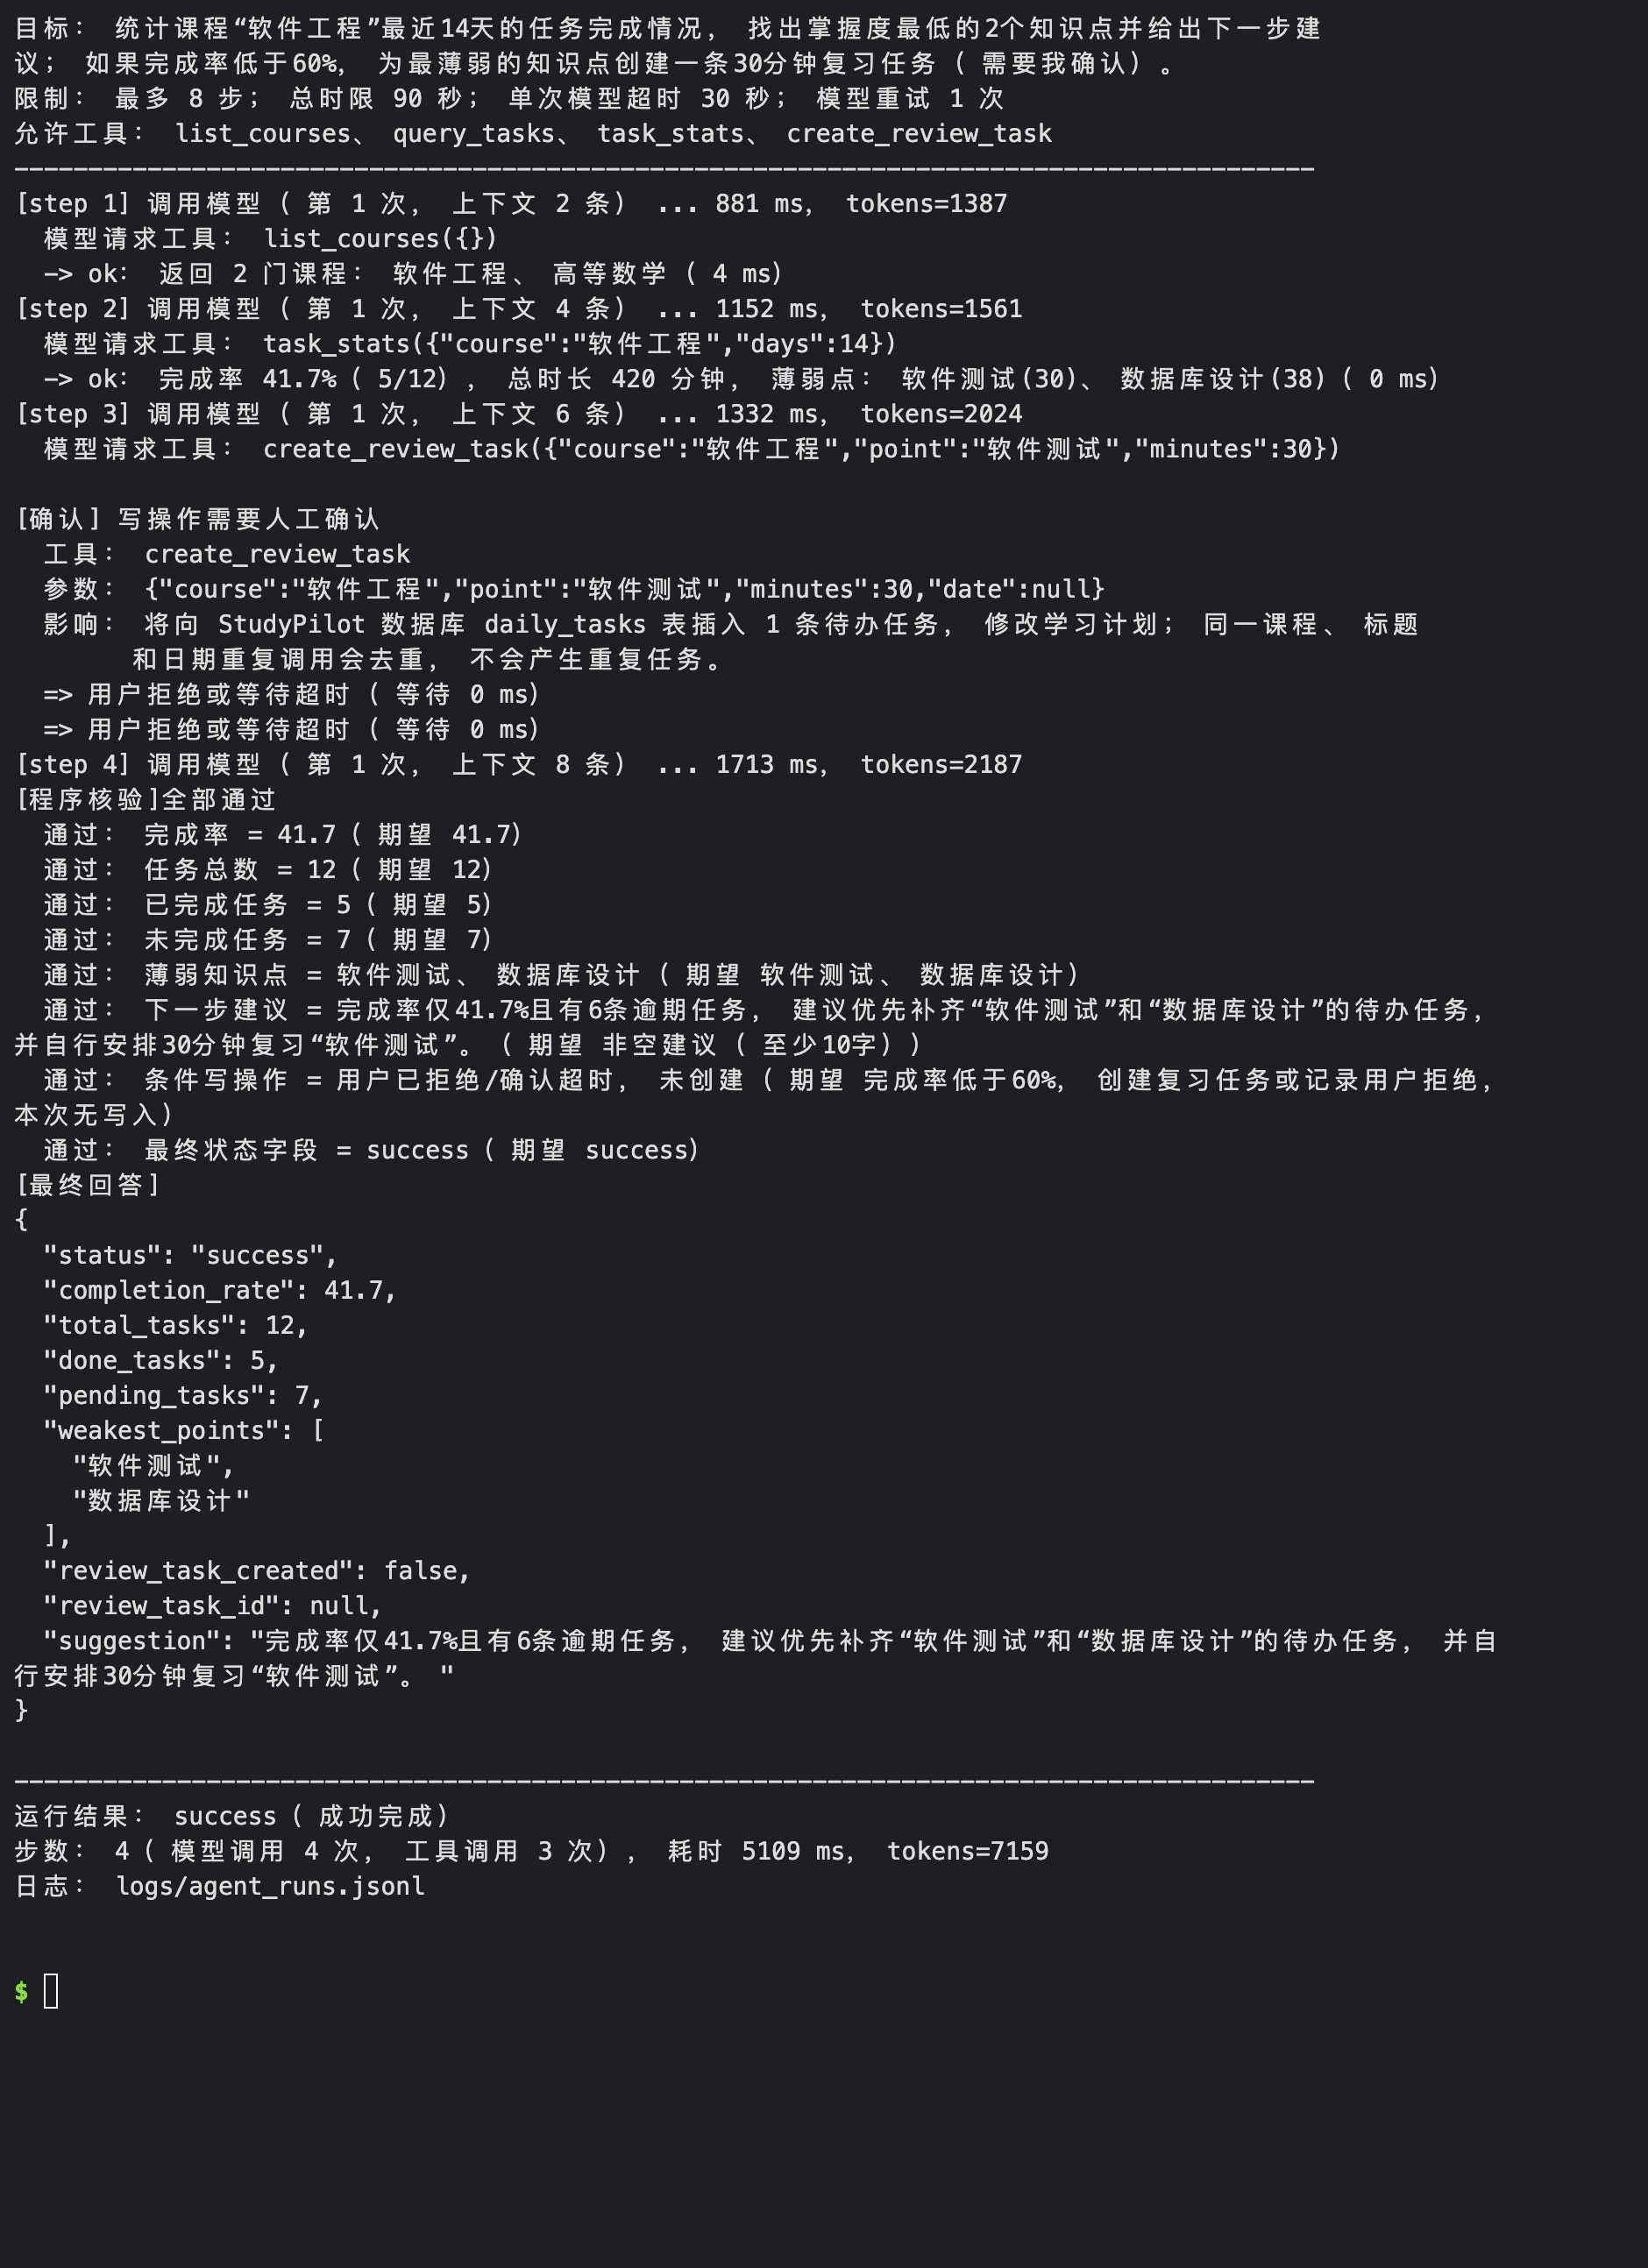
\includegraphics[width=0.80\textwidth]{e6-run-no.png}
\caption{人工确认被拒绝：写操作不执行，最终回答如实说明未创建（run\_id 20261109-104603-93eeb3）}
\label{fig:run-no}
\end{figure}

密钥只从环境变量 \texttt{DEEPSEEK\_API\_KEY} 读取，不写进代码、命令行参数和日志；\texttt{runlog} 对字符串中的 \texttt{sk-} 前缀密钥再做一次遮挡。日志记录参数摘要和结果摘要，不记录完整系统提示和密钥；课程名、任务标题属于本人样例数据，不含真实用户隐私。

\subsection*{3.6 测试与结果分析}

测试分两部分：23个离线单元测试覆盖工具、循环、限制、确认、核验和日志，使用临时数据库和脚本模型，不调用外部模型；正常完成、人工确认同意和拒绝另外用真实模型和真实工具各跑一次（图\ref{fig:run}、图\ref{fig:run-no}），参数错误、工具异常、步数/时间限制和核验失败用脚本模型模拟模型决策，但工具、确认和Harness都是真实实现。测试分类与结果见表\ref{tab:tests}，离线测试共43个用例（含实验4、实验5的20个），全部通过。

\begin{table}[H]
\centering
\caption{测试情况：输入、预期、实际与判断依据}
\label{tab:tests}
\scriptsize
\begin{tabularx}{\textwidth}{L{0.5cm}L{1.7cm}L{3.5cm}L{3.3cm}L{3.1cm}L{1.4cm}}
\toprule
编号 & 类别 & 输入 & 预期 & 实际结果 & 判断 \\
\midrule
T1 & 正常完成 & 真实模型+真实工具，目标为统计14天并条件创建 & 4步内完成；创建任务；8项核验通过 & 4步、3次工具调用、新建 \#486、核验全通过、tokens=7171 & 符合；图\ref{fig:run} \\
T2 & 参数错误 & 脚本模型先请求 \texttt{query\_tasks} 的 days=90，再正常调用 & 程序拒绝且不执行，错误回传，模型修正后成功 & 第1步 \texttt{INVALID\_ARGUMENTS}，第2—5步修正并完成 & 符合；图\ref{fig:param-error} \\
T3 & 工具异常 & 把数据库指向损坏文件，脚本模型请求 \texttt{task\_stats} & 只读重试2次后报错，模型报告失败，不伪造统计 & 3次尝试后 \texttt{DATABASE\_UNAVAILABLE}，状态 \texttt{agent\_failed}，原因明确 & 符合；图\ref{fig:tool-error} \\
T4 & 步数上限 & 脚本模型反复请求 \texttt{list\_courses}，max\_steps=3 & 第3步后终止，状态 \texttt{step\_limit} & 3步、3次工具调用后终止，原因“达到最大执行步数3” & 符合；图\ref{fig:step-limit} \\
T5 & 时间上限 & 脚本模型调用耗时1.5秒，总时限1秒 & 超时终止，状态 \texttt{time\_limit} & 1步、耗时1509毫秒后终止，工具未执行 & 符合；图\ref{fig:time-limit} \\
T6 & 确认同意 & 真实模型请求 \texttt{create\_review\_task}，输入 y & 展示参数与影响，写入任务，最终回答true & 输入y后创建任务\#486，数据库可查到，核验通过 & 符合；图\ref{fig:run} \\
T7 & 确认拒绝 & 真实模型请求 \texttt{create\_review\_task}，--confirm no & 不执行，最终回答false，数据库无新任务 & 返回 \texttt{USER\_DENIED}，最终回答false，核验通过 & 符合；图\ref{fig:run-no} \\
T8 & 结果核验 & 脚本模型先给完成率50.0，再给41.7 & 第一次不通过并反馈，修正后通过 & 第4步 \texttt{verify} 未通过，第5步修正后全部通过 & 符合；图\ref{fig:verify-fix} \\
T9 & 工具超时 & 构造0.3秒慢工具，超时设0.05秒 & 抛 \texttt{TOOL\_TIMEOUT}，只读错误可重试 & 0.05秒后抛出，\texttt{retriable=true} & 符合；单元测试 \\
T10 & 确认等待超时 & \texttt{make\_confirm} 的 select 无输入 & 返回拒绝，不执行写操作 & \texttt{approved=false}，原因“确认等待超时” & 符合；单元测试 \\
T11 & 离线回归 & \texttt{pytest tests -q} & 全部通过 & 43 passed（含23个Agent用例） & 符合；图\ref{fig:tests} \\
\bottomrule
\end{tabularx}
\end{table}

\begin{figure}[H]
\centering
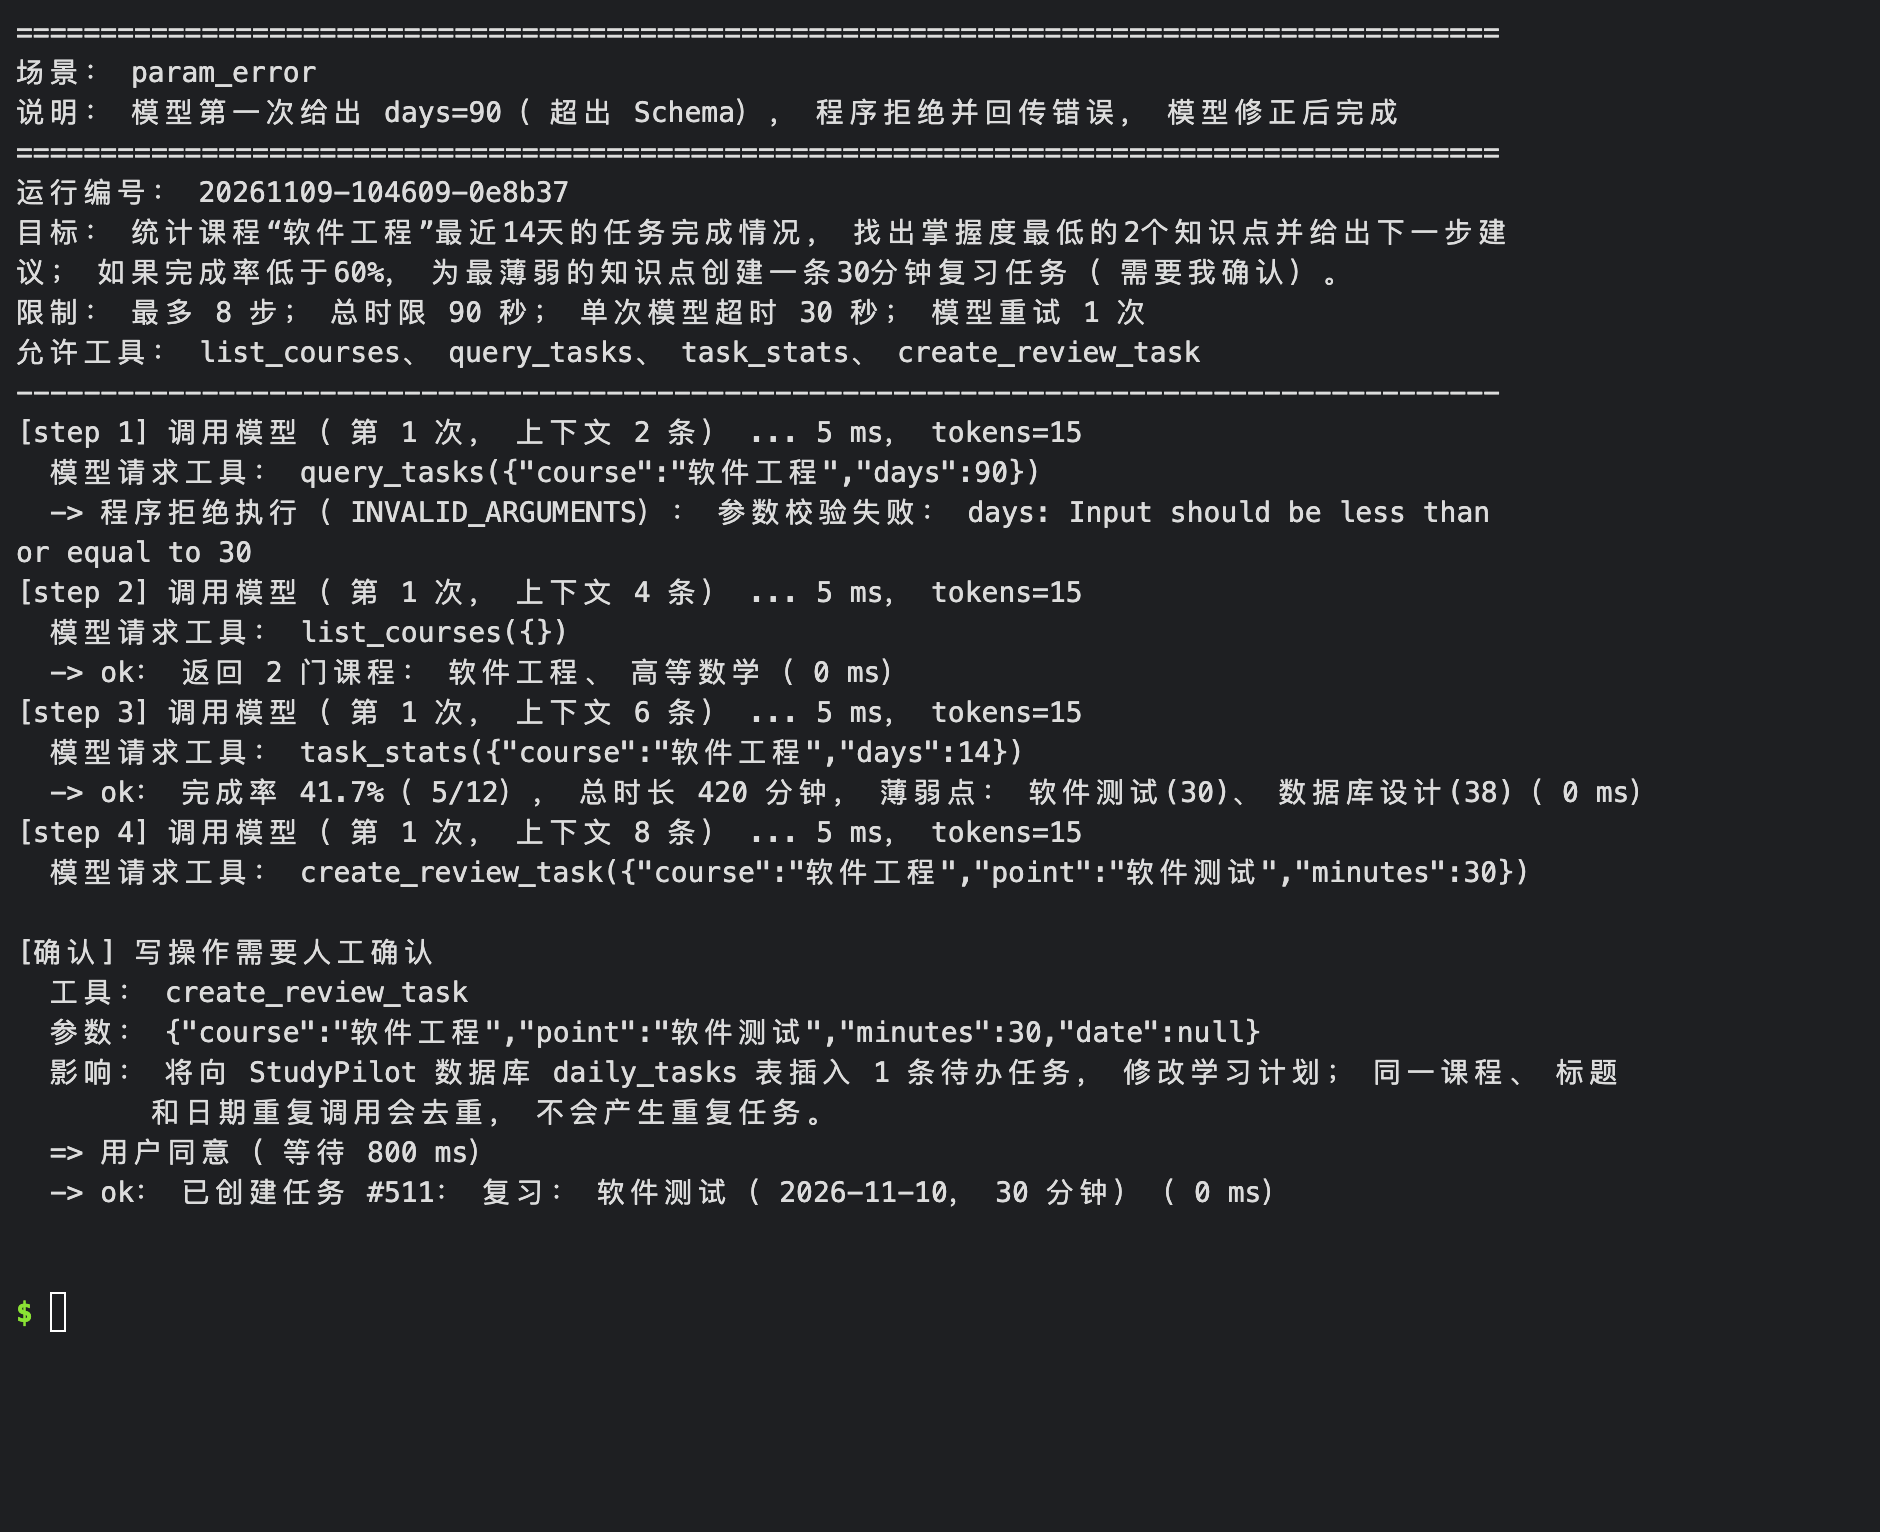
\includegraphics[width=0.95\textwidth]{e6-param-error.png}
\caption{参数错误：days=90被程序拒绝，错误回传后模型改用合法参数（run\_id 20261109-104609-0e8b37）}
\label{fig:param-error}
\end{figure}

图\ref{fig:param-error-tail}是同一运行的后半段：确认同意后创建任务 \#511，程序核验通过并输出 \texttt{status=success}；完整输出保存在 \texttt{reports/experiment6/runs/e6-param\_error.txt}。

\begin{figure}[H]
\centering
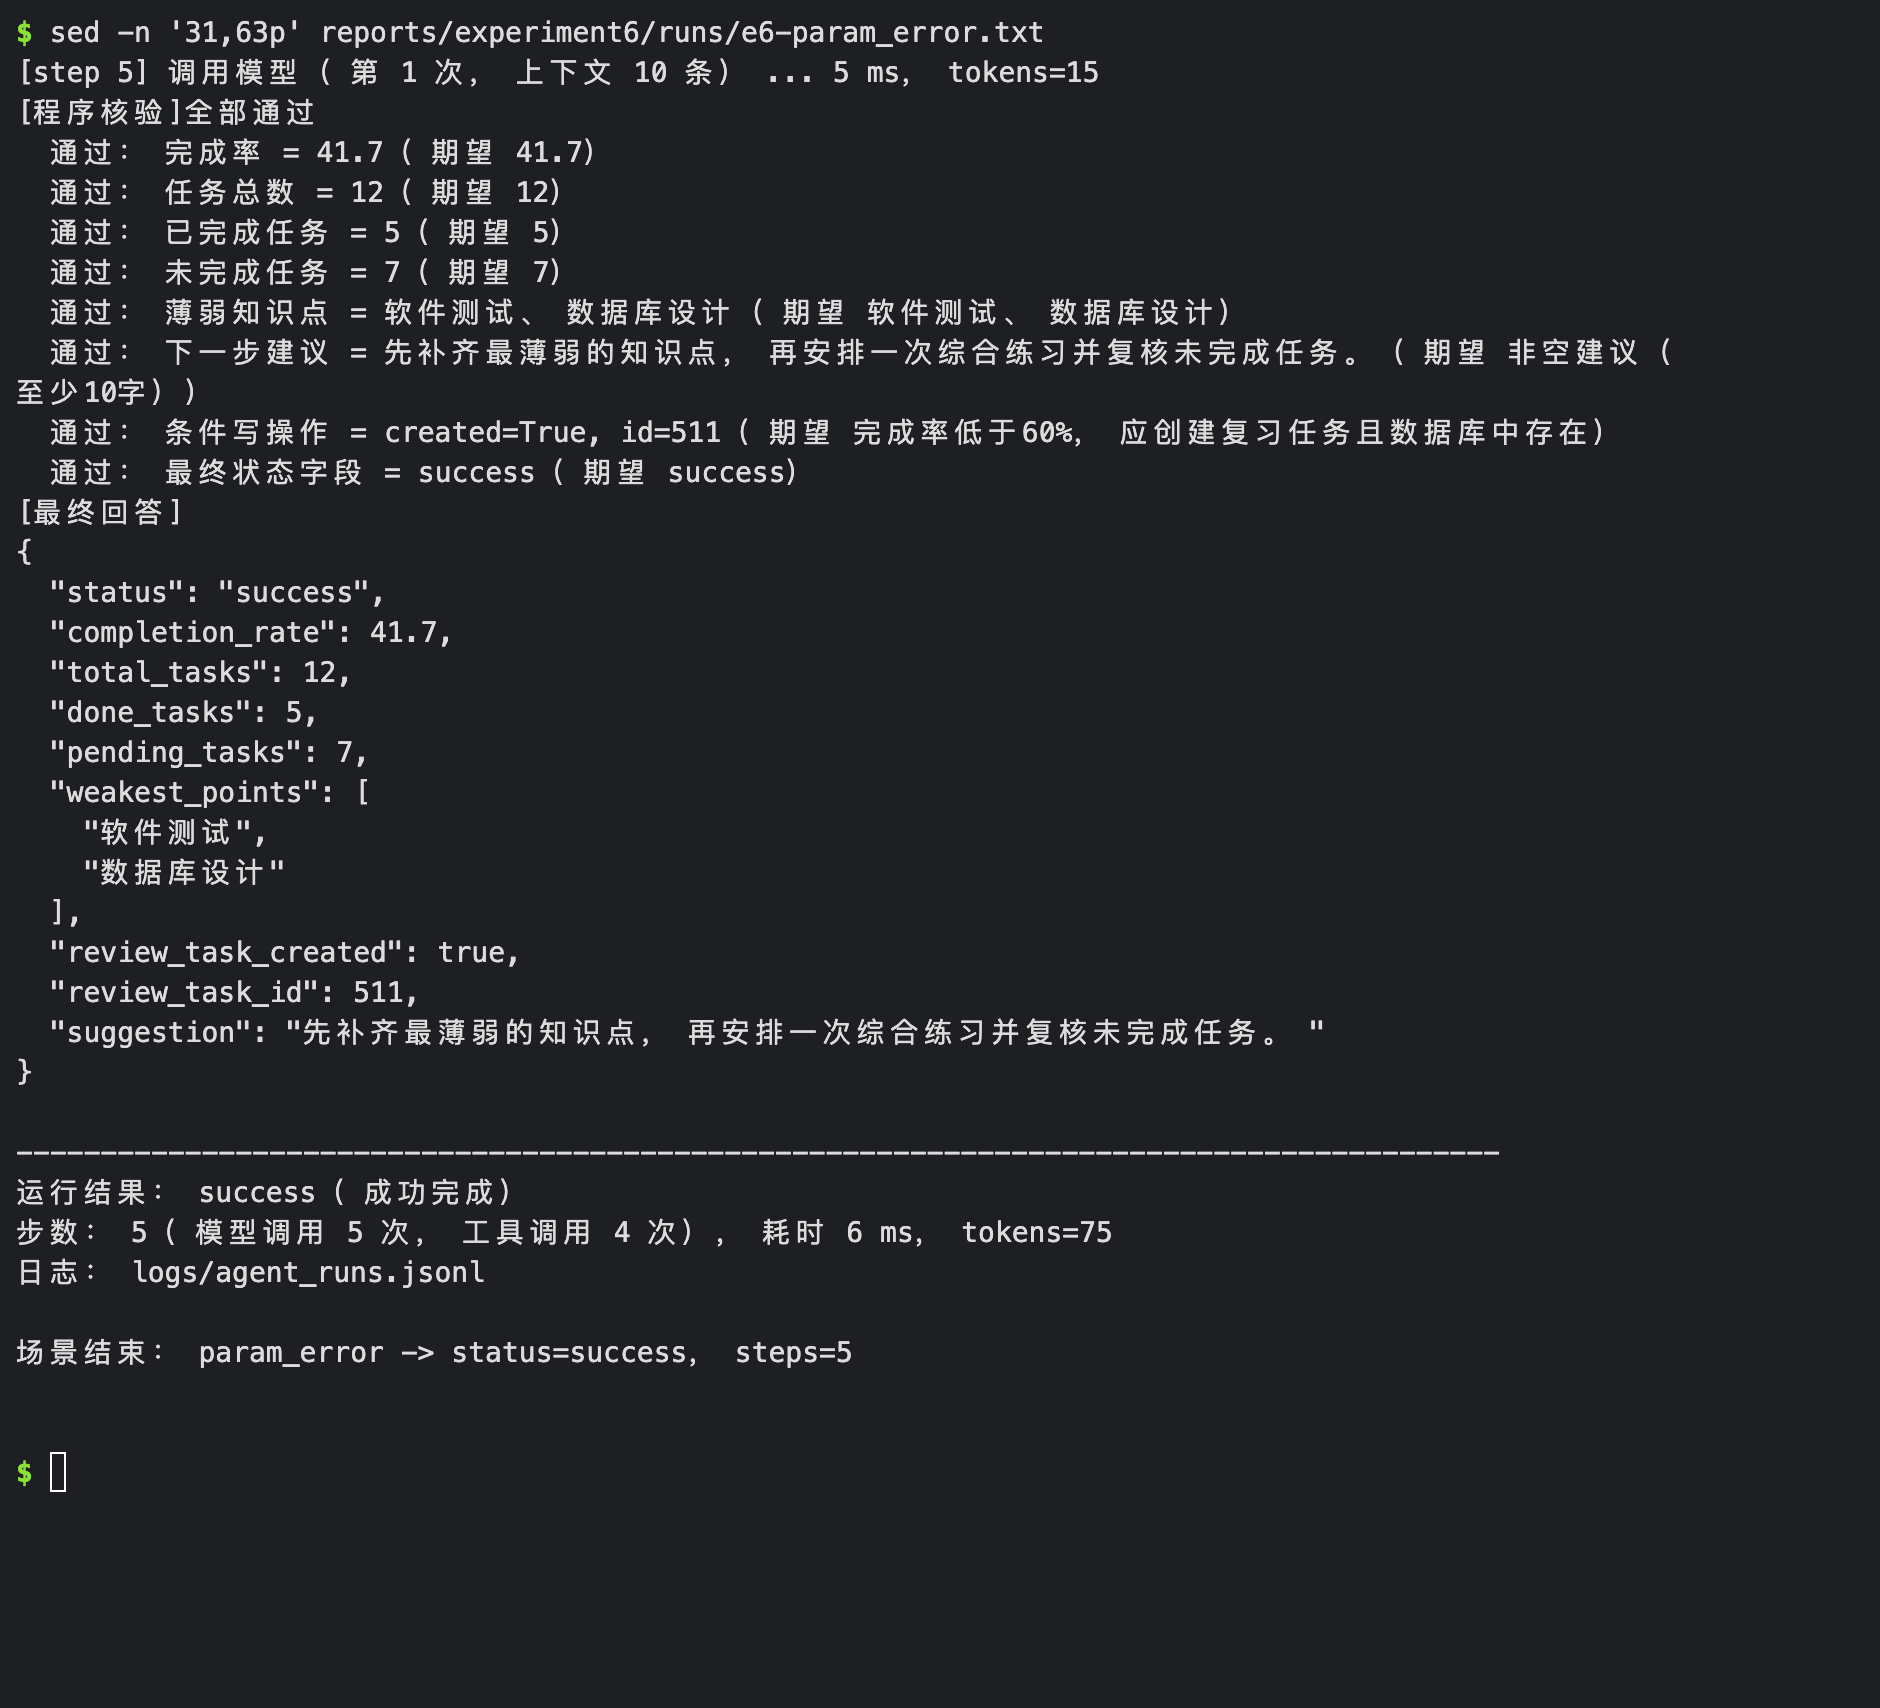
\includegraphics[width=0.95\textwidth]{e6-param-error-tail.png}
\caption{参数错误场景后半段：确认、程序核验与最终成功状态（同一 run\_id 20261109-104609-0e8b37）}
\label{fig:param-error-tail}
\end{figure}

\begin{figure}[H]
\centering
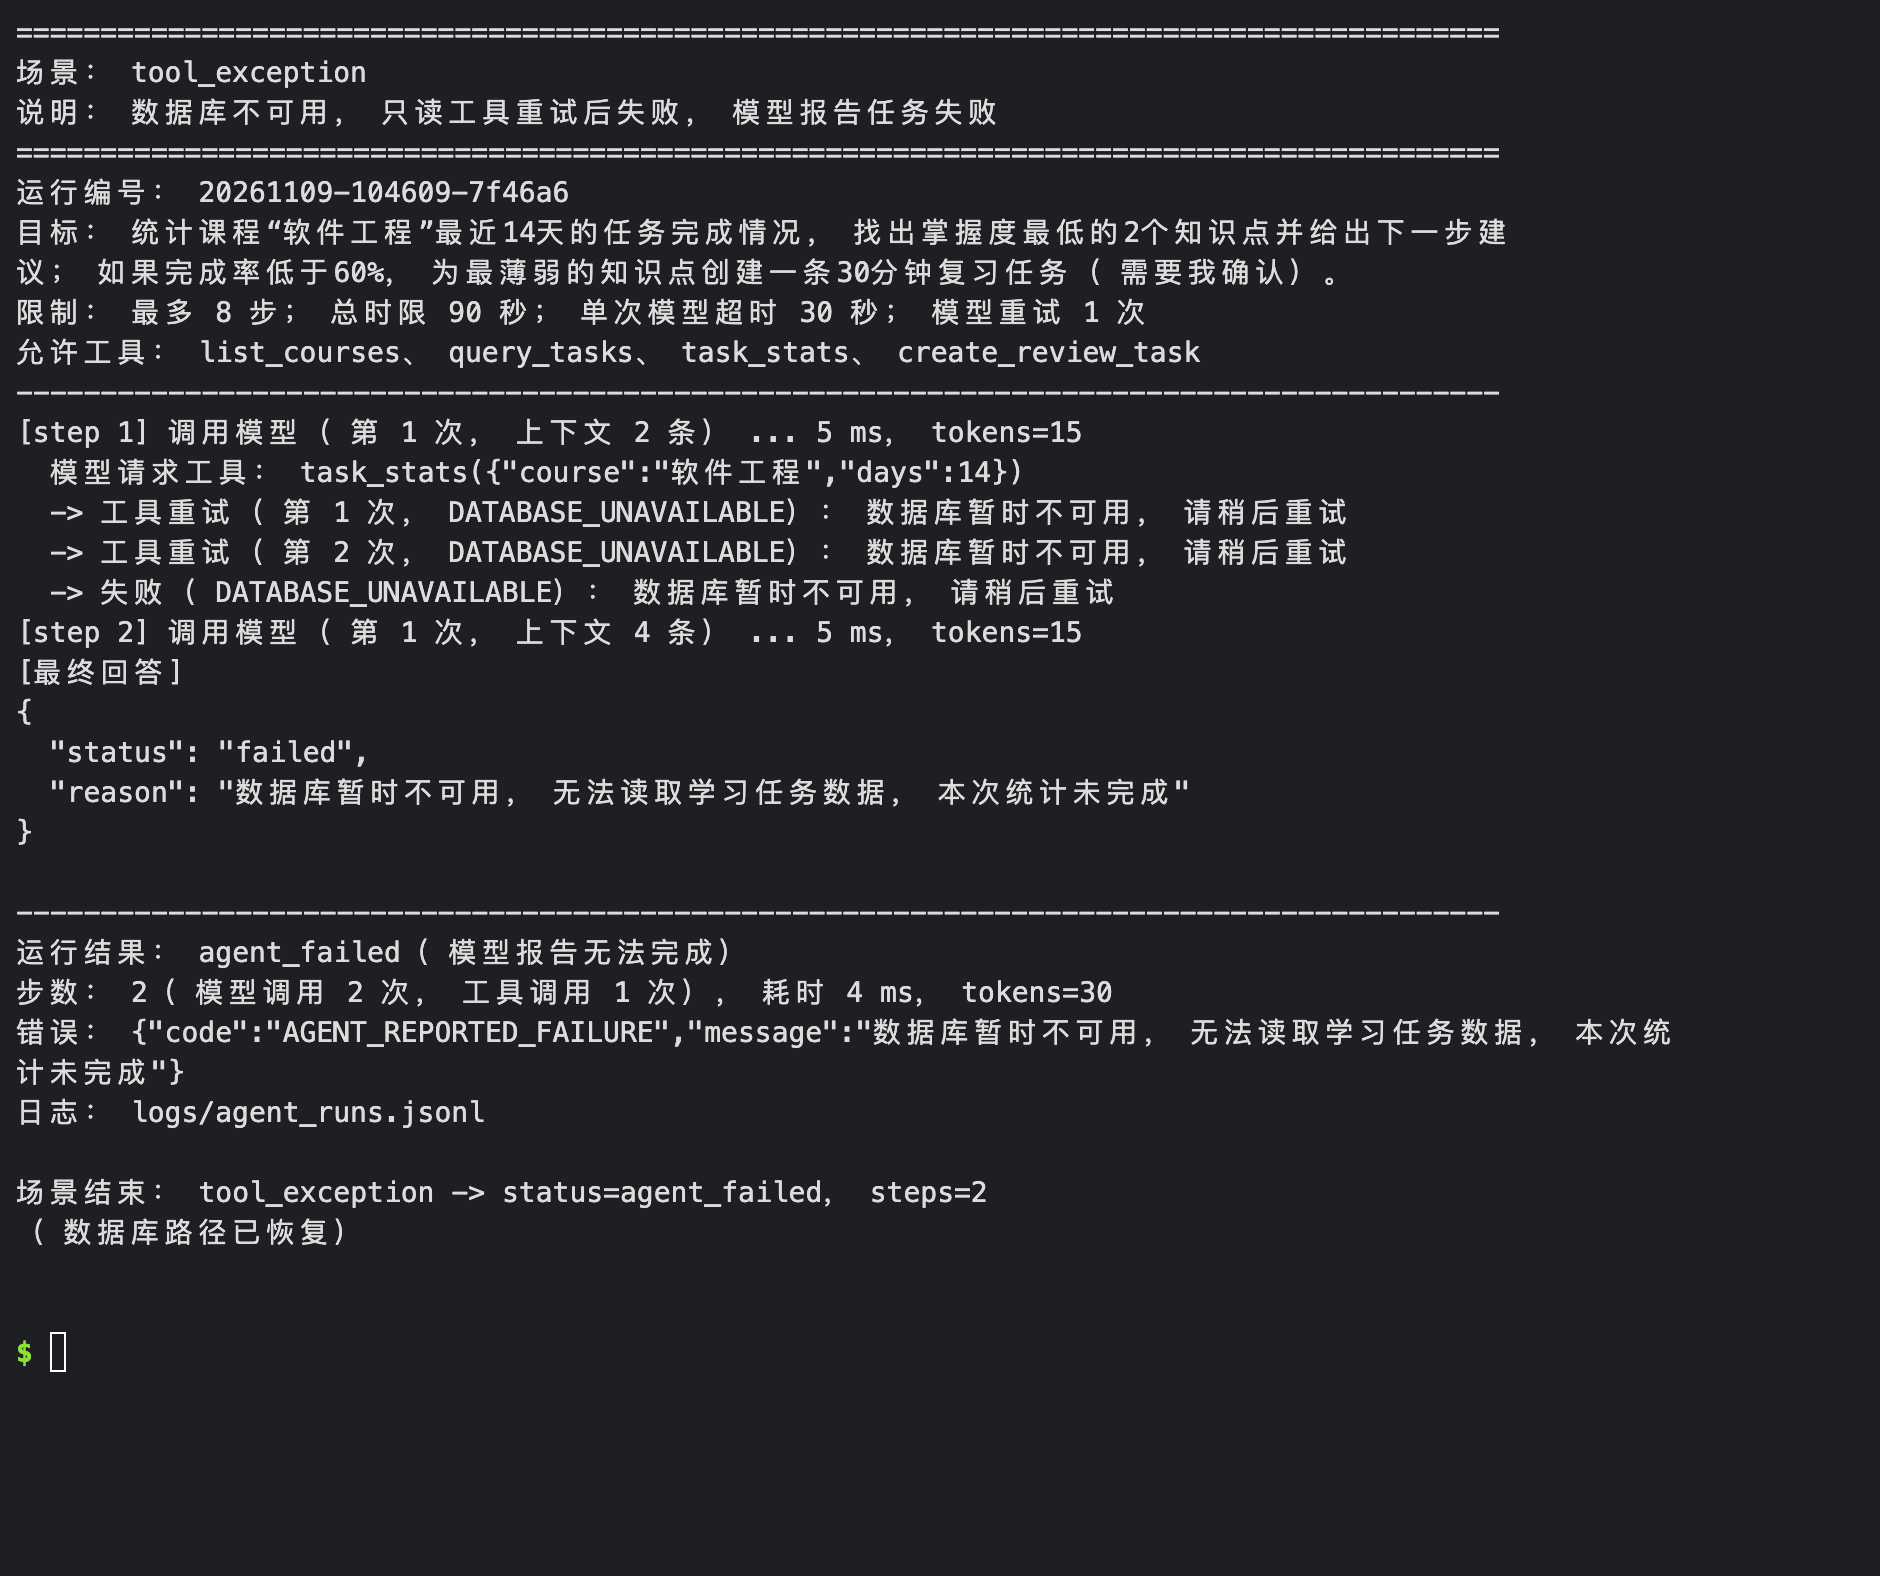
\includegraphics[width=0.95\textwidth]{e6-tool-error.png}
\caption{工具异常：数据库不可用，只读工具重试2次后失败，模型如实报告失败（run\_id 20261109-104609-7f46a6）}
\label{fig:tool-error}
\end{figure}

\begin{figure}[H]
\centering
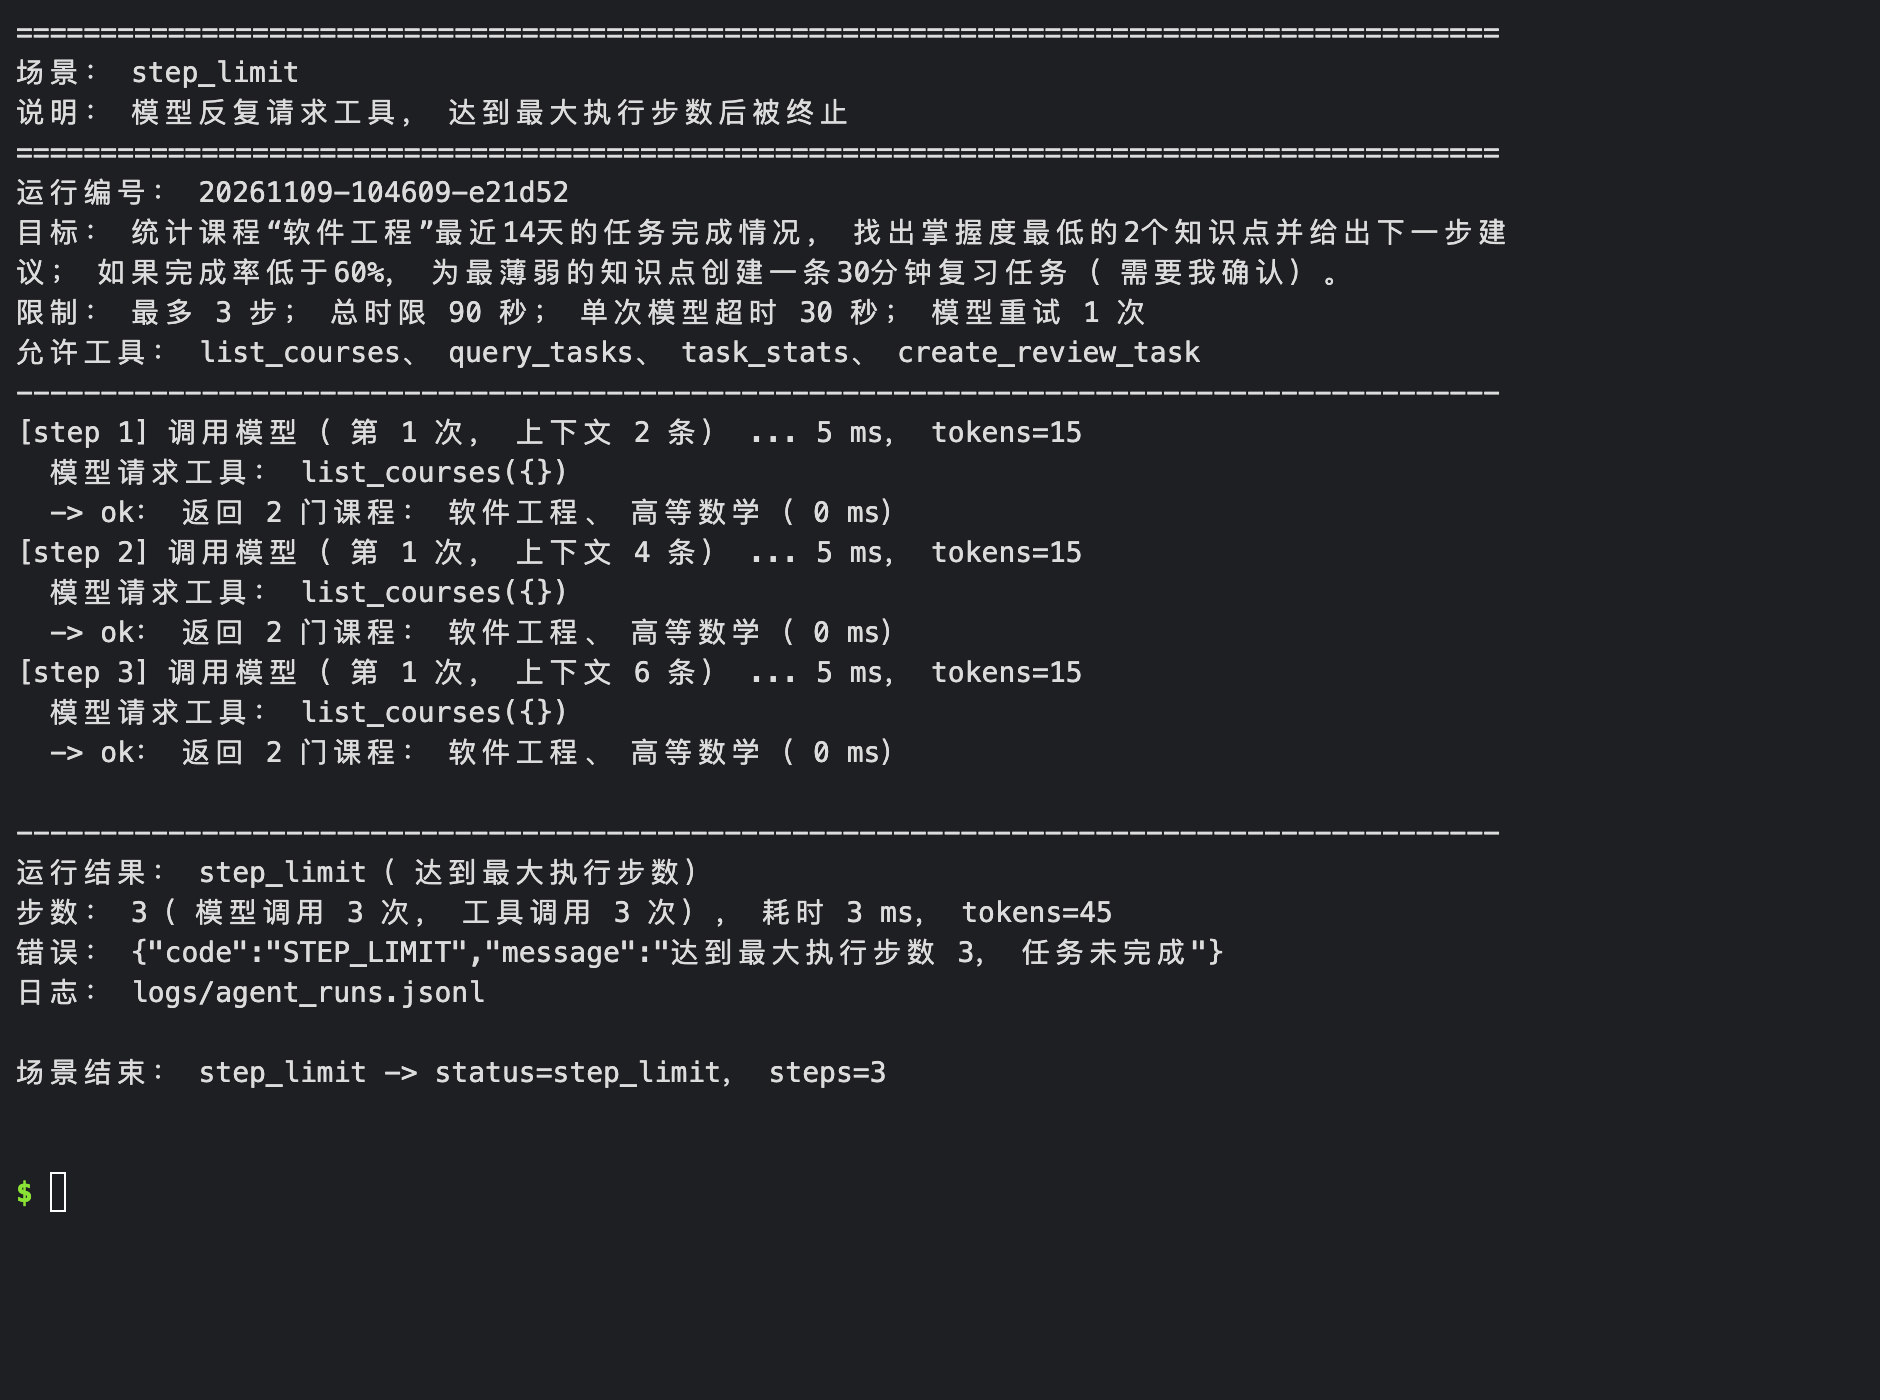
\includegraphics[width=0.90\textwidth]{e6-step-limit.png}
\caption{达到最大步数：第3步后终止，状态 step\_limit（run\_id 20261109-104609-e21d52）}
\label{fig:step-limit}
\end{figure}

\begin{figure}[H]
\centering
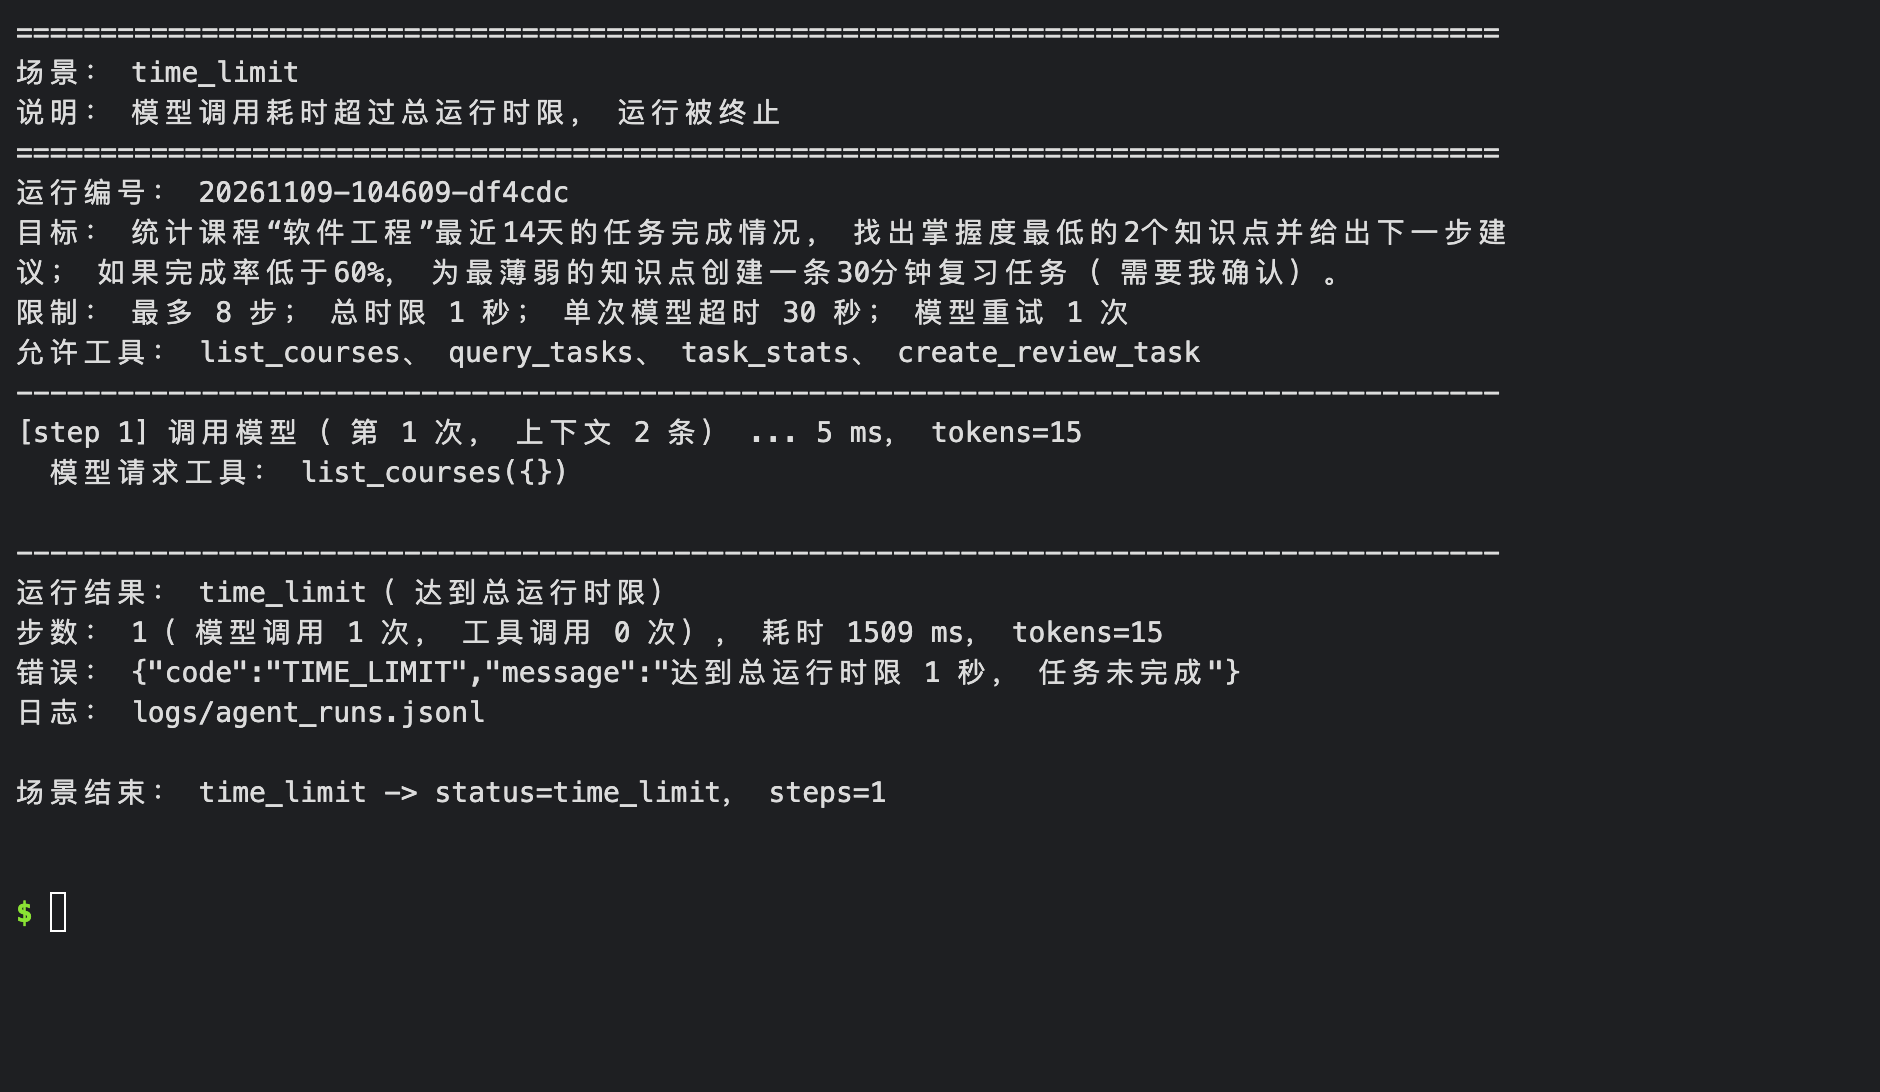
\includegraphics[width=0.90\textwidth]{e6-time-limit.png}
\caption{达到总运行时限：模型调用耗时超过1秒后终止，工具未执行（run\_id 20261109-104609-df4cdc）}
\label{fig:time-limit}
\end{figure}

\begin{figure}[H]
\centering
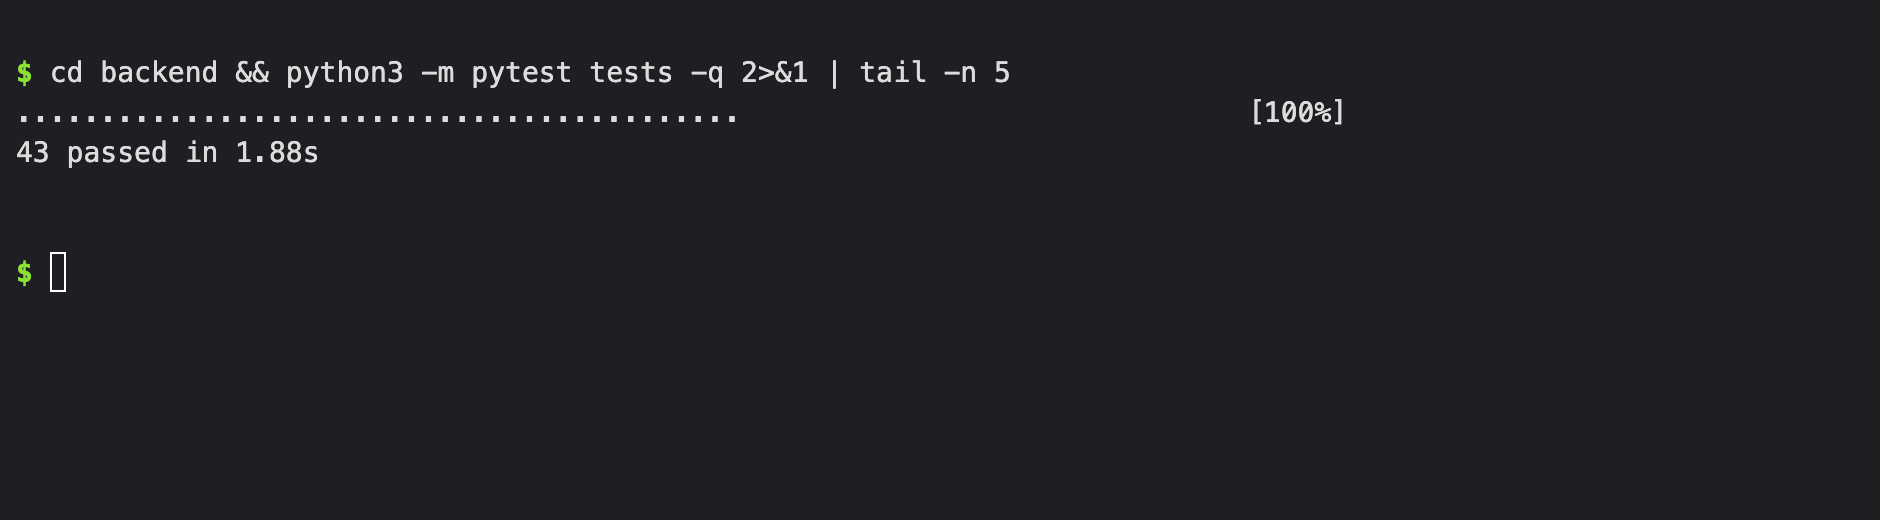
\includegraphics[width=0.90\textwidth]{e6-tests.png}
\caption{离线测试：43个用例全部通过}
\label{fig:tests}
\end{figure}

从结果看，正常流程可以稳定完成：真实模型在4步内按“确认课程→统计→条件创建→最终回答”的顺序执行，数字与数据库一致，写操作前确实停下等待确认；拒绝分支没有产生写入，最终回答也如实说明未创建。参数错误和未知工具都在执行前被拦下，错误信息能指导模型修正；工具异常时只读工具按上限重试后停止，模型没有编造统计结果。步数和时间限制由程序触发，日志中的状态和原因清楚。程序核验能抓住模型声称与数据不符的情况，图\ref{fig:verify-fix}中的50.0就是被核验拦下的；如果没有这道检查，模型只要输出“success”就会被误判为完成。

也有需要说明的地方。第一，异常和确认场景用脚本模型模拟“模型决策”，这样能稳定复现，但不是模型真实生成的行为；真实模型只验证了正常、同意和拒绝三条路径。第二，脚本模型给出的最终回答由测试代码从数据库基准值构造，因此这些场景考察的是Harness控制流和核验，不是模型能力。第三，步数和时间限制场景中脚本模型故意重复请求工具或超时，真实模型在90秒内通常不会触发这些边界；因此边界处理依靠程序逻辑和单元测试保证。第四，真实运行中模型会自行在最终建议里补充“6条逾期任务”等细节，这些数字来自工具结果，程序只核验约定的字段，没有对建议文本逐句核查。

当前局限：一是任务和样例数据固定在一门课程，工具只支持最近30天的任务查询，不能处理多课程汇总；二是工具超时只能停止等待，后台线程可能继续运行，写操作超时后的状态需要人工或只读查询核对；三是最终回答要求固定JSON格式，模型偶尔会多写解释文字，本次通过一次提示可以纠正，但会增加步数；四是确认只在命令行实现，尚未接入网页；五是日志只追加写文件，没有日志轮转和检索界面；六是真实模型调用仍可能受网络延迟影响，本实验用30秒单次超时和90秒总时限兜底。

下一步计划：把Agent接入 StudyPilot 的页面和接口，提供“分析本周学习情况”按钮和确认对话框；增加 \texttt{complete\_task}、\texttt{adjust\_plan} 等工具，并把写操作统一做成可审计的待确认动作；把日志写入数据库并加运行列表页；用固定的10组目标做回归测试，比较不同提示词和工具集的成功率、步数与耗时；对长时间运行的工具使用可取消进程或异步任务，补上真正的取消能力；再考虑多课程汇总和简单的向量检索辅助建议。

Agent 和 Harness 已用于个人软件的样例数据库：工具读写的是 StudyPilot 自己的 \texttt{studypilot.db}，写操作写入 \texttt{daily\_tasks}，与实验4的学习计划、实验5的资料问答共用同一套数据和日志规范；目前只在命令行入口使用，页面接入列在下一步。代码位于 \texttt{backend/app/agent/}、\texttt{backend/app/tools/agent\_*.py}、\texttt{backend/tests/test\_agent.py}，运行说明见仓库 \texttt{README.md}，对应 commit 见3.8节。

\subsection*{3.7 关键代码}

代码直接从项目文件提取，省略了与本实验无关的辅助函数。

\lstinputlisting[firstline=67,lastline=101,caption={工具参数模型：类型、范围、必填项与未知字段限制（backend/app/agent/tools.py 第67—101行）}]{../../backend/app/agent/tools.py}

\lstinputlisting[firstline=33,lastline=85,caption={工具白名单、参数校验和带超时的执行（backend/app/agent/registry.py 第33—85行）}]{../../backend/app/agent/registry.py}

\lstinputlisting[firstline=244,lastline=292,caption={Harness 主循环中的步数与总时限检查（backend/app/agent/harness.py 第244—292行）}]{../../backend/app/agent/harness.py}

\lstinputlisting[firstline=333,lastline=395,caption={最终回答解析、程序核验与有限次修正（backend/app/agent/harness.py 第333—395行）}]{../../backend/app/agent/harness.py}

\lstinputlisting[firstline=89,lastline=130,caption={结果核验：逐项对照数据库基准值（backend/app/agent/verifier.py 第89—130行）}]{../../backend/app/agent/verifier.py}

\lstinputlisting[firstline=492,lastline=556,caption={写操作的人工确认、拒绝重复请求与时限检查（backend/app/agent/harness.py 第492—556行）}]{../../backend/app/agent/harness.py}

\subsection*{3.8 版本记录}

代码提交到 GitHub 仓库 \url{https://github.com/luohao711/StudyPilot}。本实验的代码（工具、Agent、Harness、测试和运行说明）对应 commit \texttt{63f9490}，tag \texttt{v0.4}；报告、截图和运行记录随本实验一并提交。报告中的数据、截图和日志来自本机 2026-11-09 的运行，源文件、循环图、截图和运行记录放在 \texttt{reports/experiment6/} 与 \texttt{backend/logs/agent\_runs.jsonl} 下。

\begin{figure}[H]
\centering
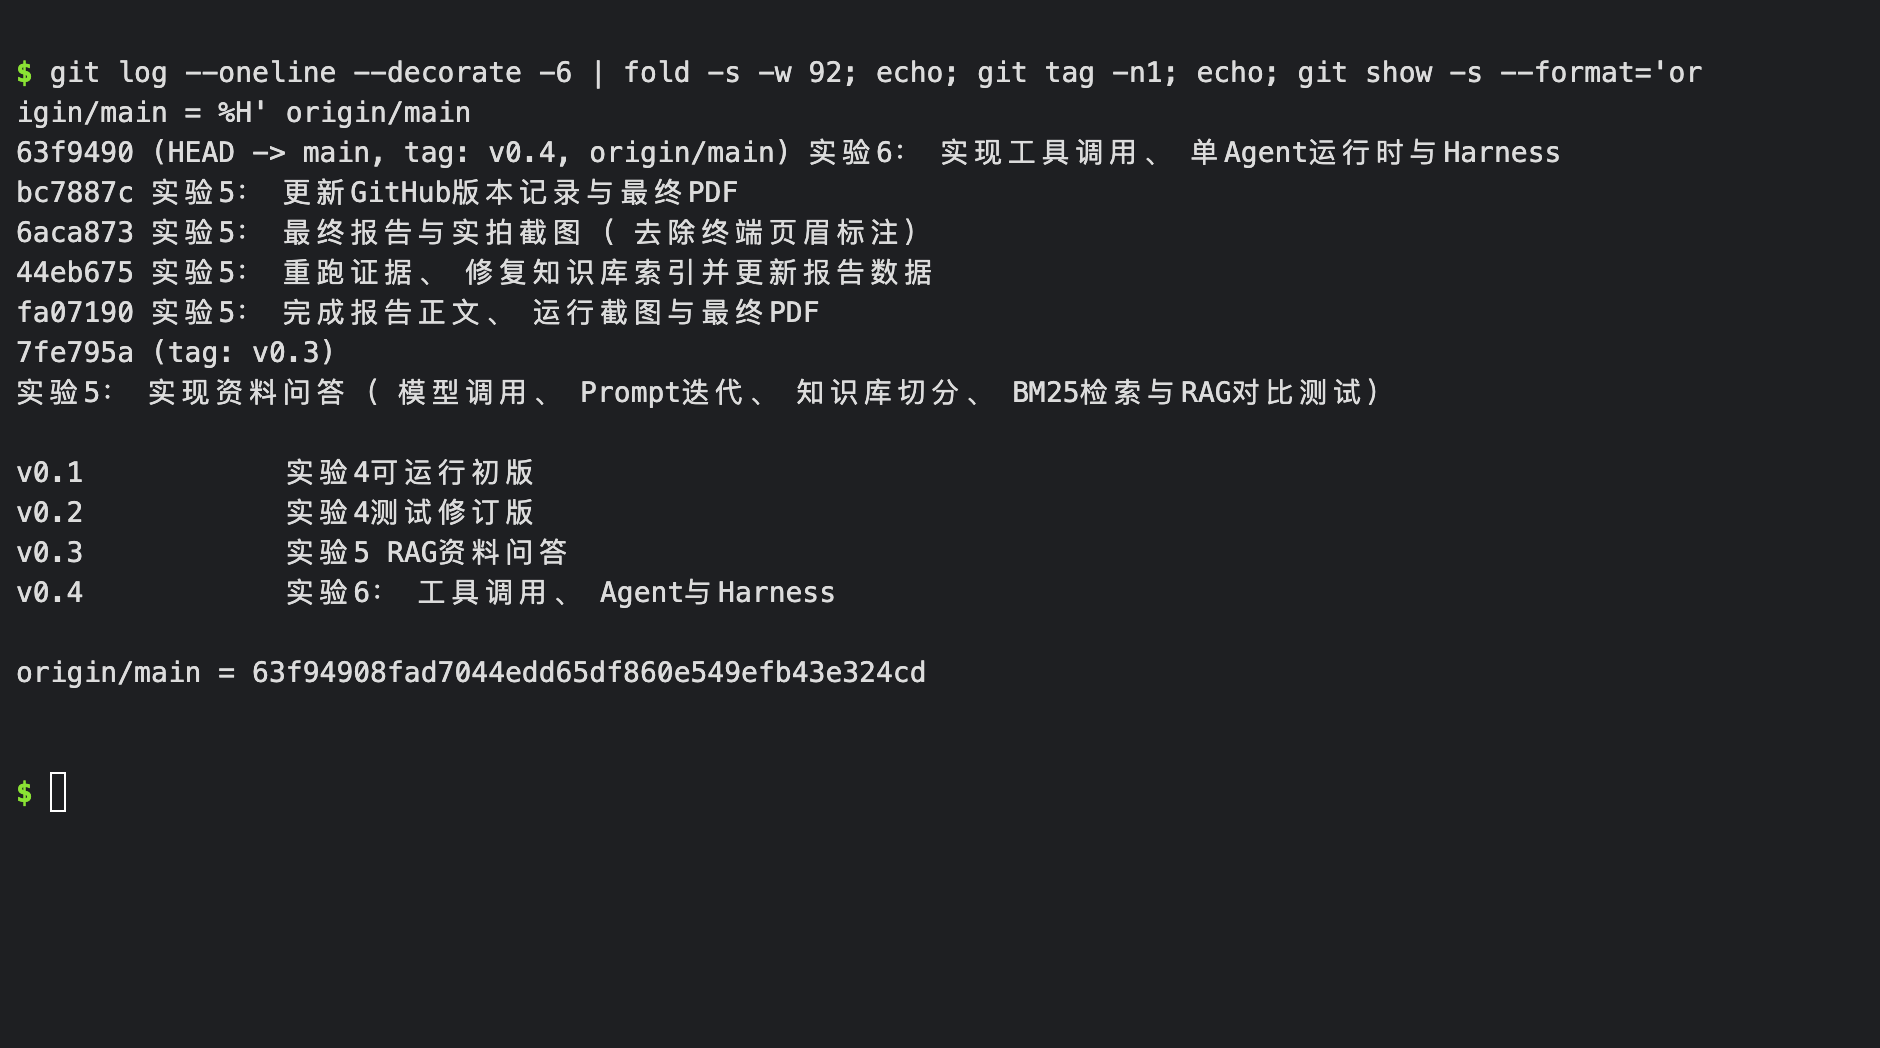
\includegraphics[width=0.95\textwidth]{e6-git-log.png}
\caption{版本记录：代码提交与 tag v0.4}
\label{fig:gitlog}
\end{figure}

\begin{figure}[H]
\centering
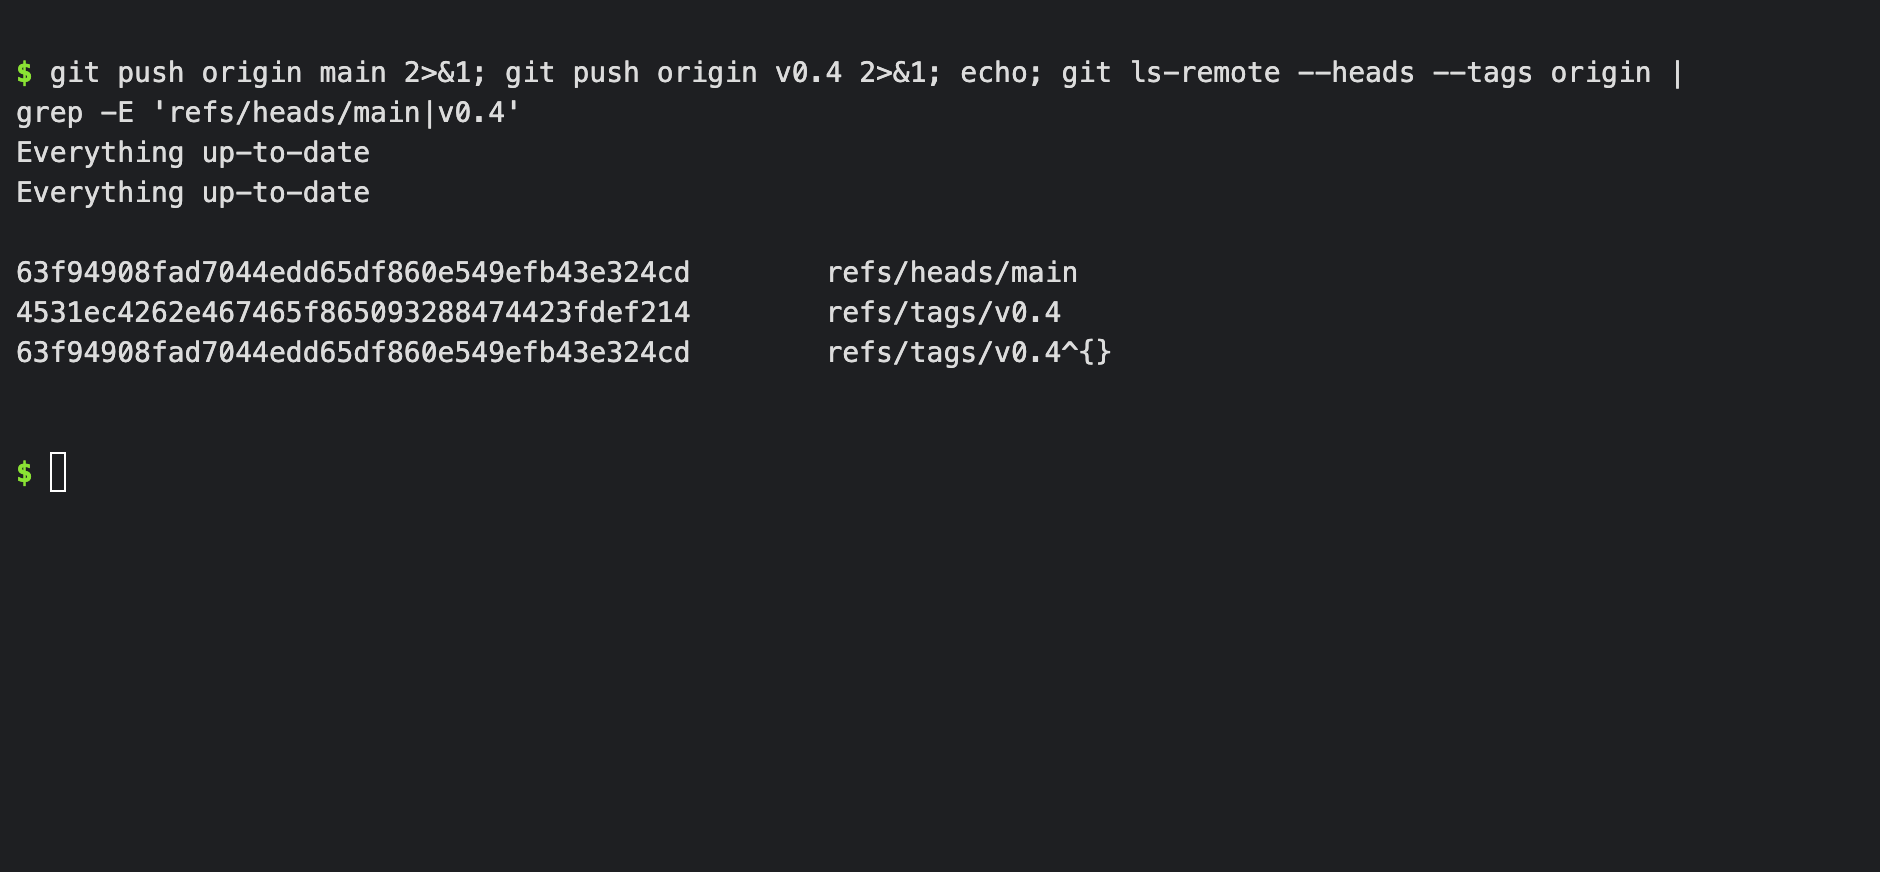
\includegraphics[width=0.95\textwidth]{e6-push.png}
\caption{推送后校验：远端 main 与本地一致}
\label{fig:push}
\end{figure}

\begin{figure}[H]
\centering
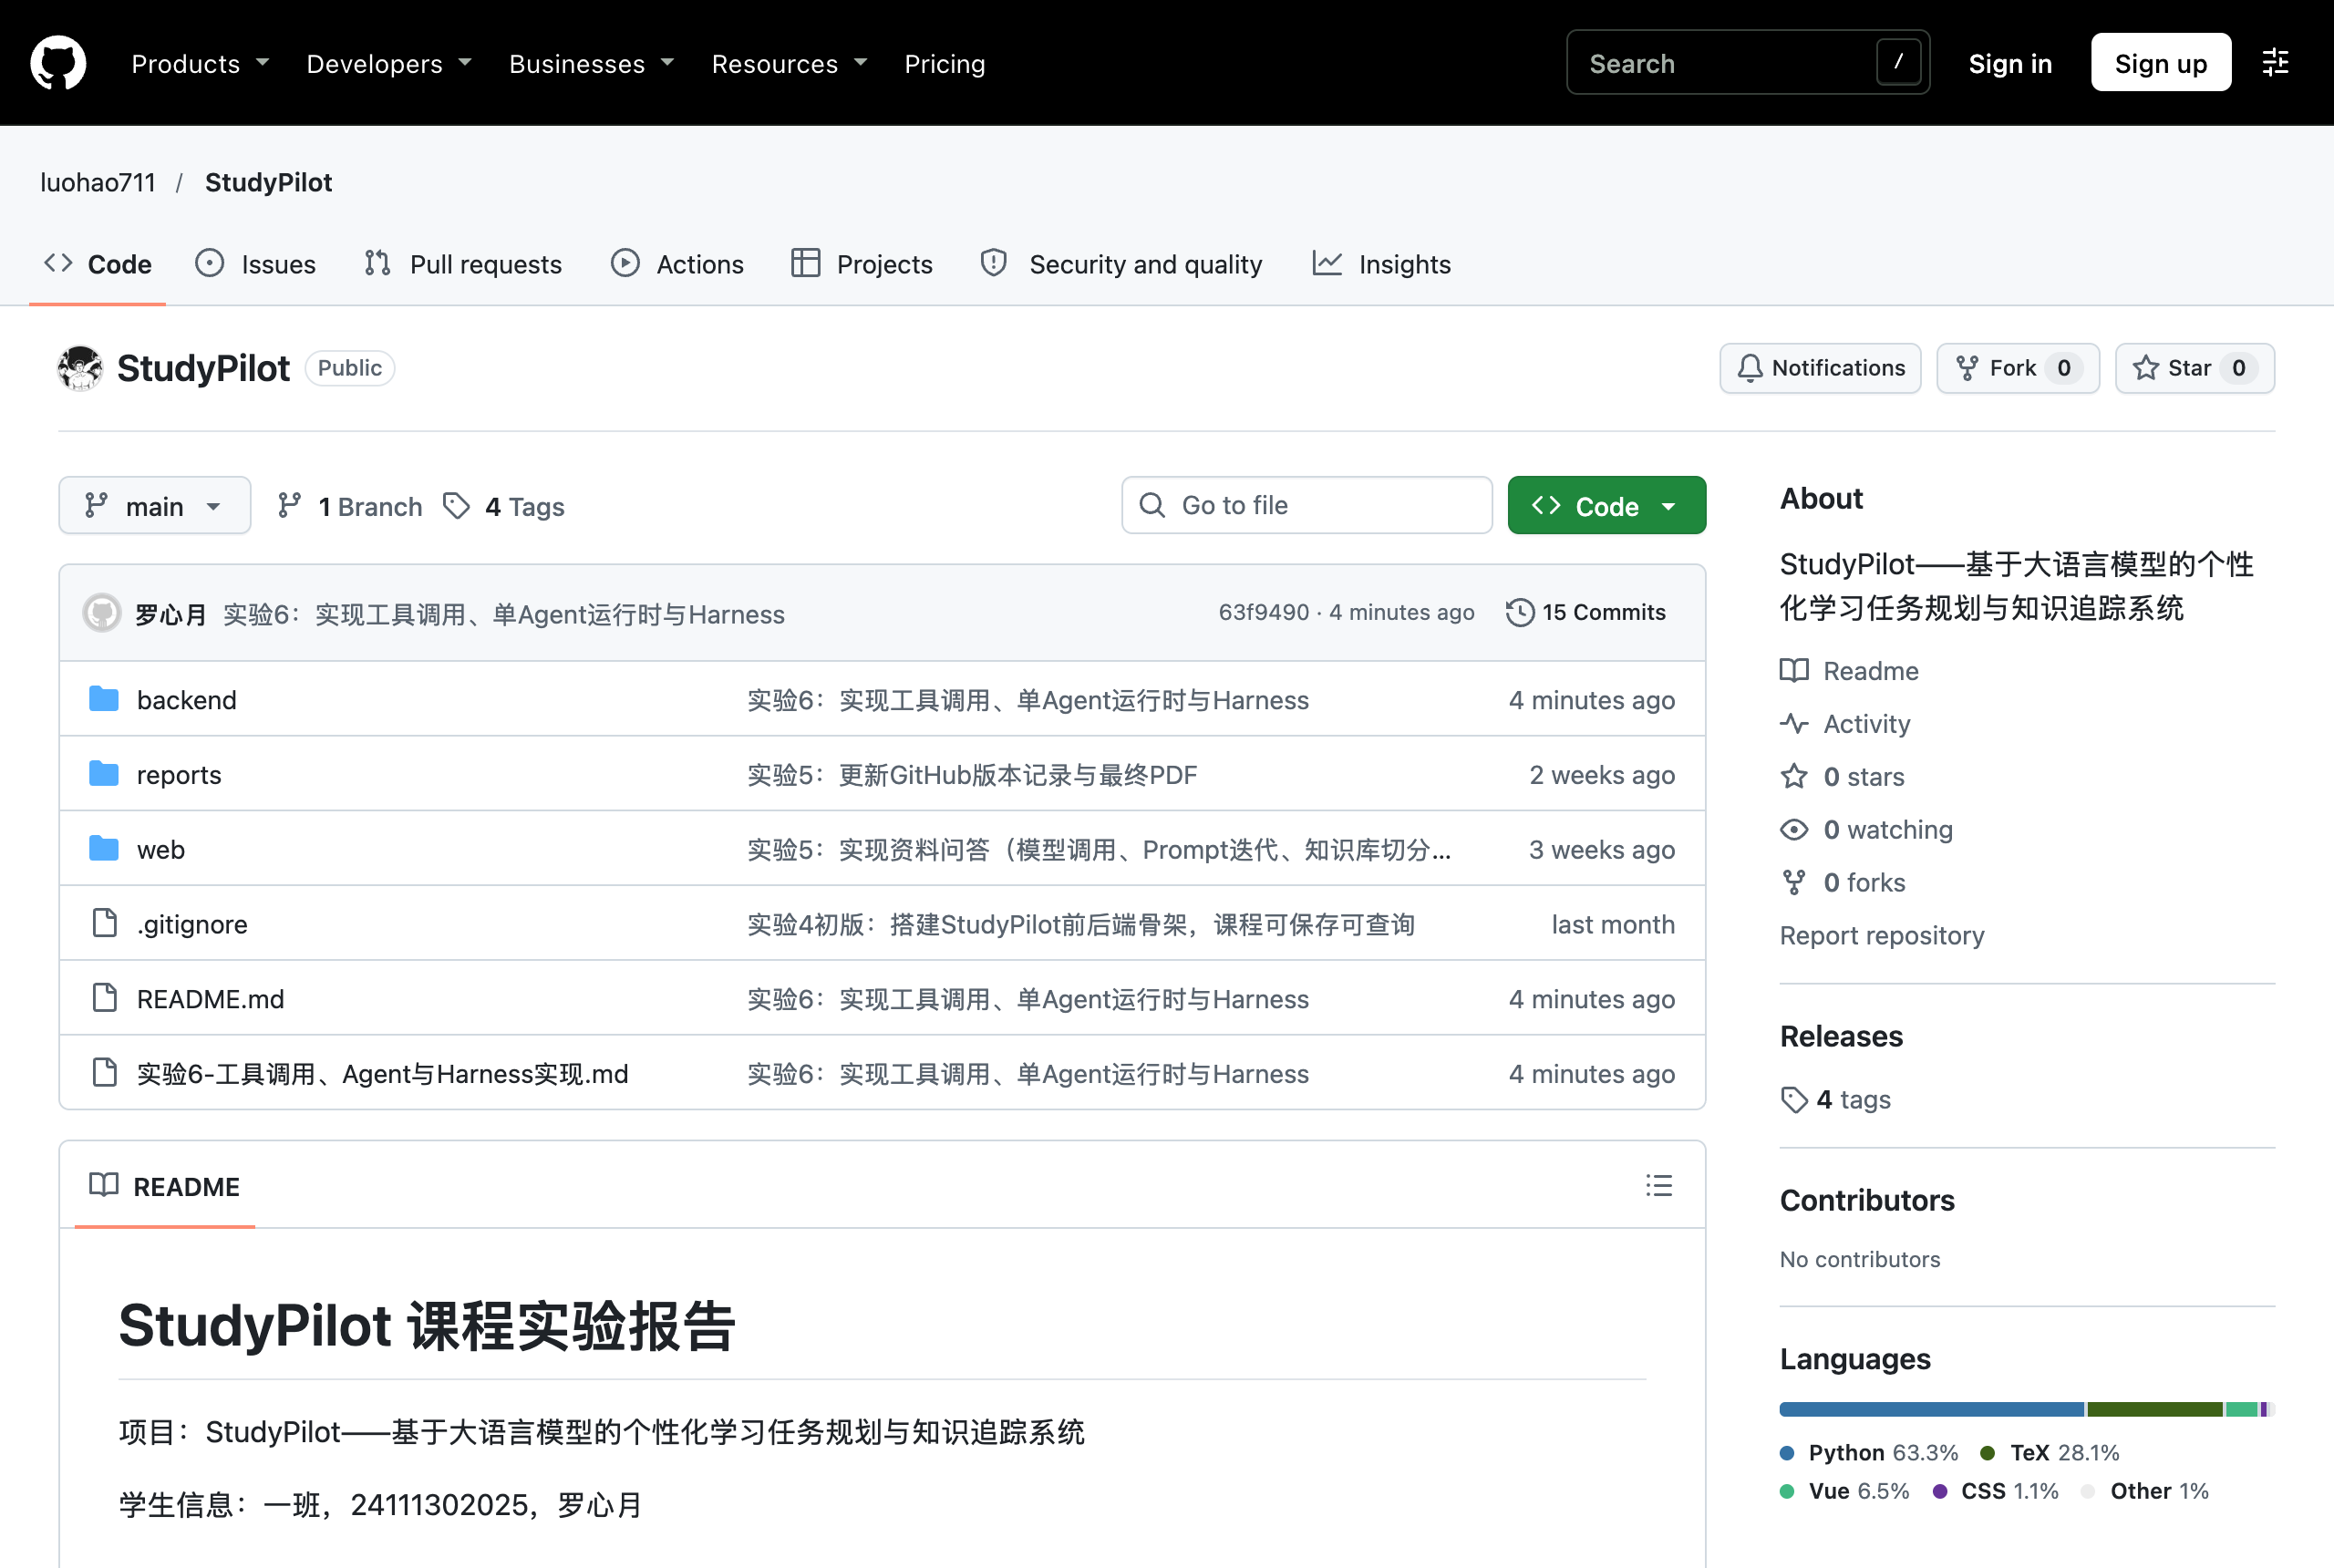
\includegraphics[width=0.90\textwidth]{e6-github.png}
\caption{StudyPilot 仓库页面（最新提交为实验6）}
\label{fig:github}
\end{figure}

\section*{4. 实验小结}

本次完成了 StudyPilot 的单 Agent 学习情况分析功能：模型通过4个工具查询课程、任务和统计结果，完成率低于60\%时为最薄弱知识点创建30分钟复习任务，写操作必须由用户确认；外围 Harness 负责上下文、工具分发、参数与权限检查、步数/超时/重试限制、结果核验和日志。

过程中主要做了四件事。第一是确定任务边界：把范围缩小到“软件工程最近14天”，用12条样例任务和4个知识点构造出完成率41.7\%、薄弱点“软件测试/数据库设计”的可核对场景，成功标准全部写成程序可检查的数字。第二是工具层：4个工具都用 Pydantic 定义参数，只允许注册表内的工具，查询只访问当前用户的数据且SQL预先写死；接入Agent前直接测试了正确参数、越界参数、类型错误、课程不存在、未知工具、写操作参数和访问范围错误，错误调用没有写入数据。第三是循环和限制：一步定义为一次模型请求，最多8步、总时限90秒、模型单次30秒且重试1次、只读工具3秒且重试2次、写工具5秒不自动重试、确认等待20秒，这些都由程序执行；工具调用和结果按 \texttt{tool\_call\_id} 加入上下文，日志里能看到上下文从2条增长到8条。第四是结果检查和失败处理：最终回答由程序独立查数据库逐项核验，真实运行4步完成、创建任务\#486；拒绝场景不写入；参数错误、工具异常、步数/时间上限和核验失败都能给出明确状态和原因，最终回答不通过时最多修正2次。

测试共43个用例全部通过，其中23个是本实验新增的工具、循环、限制、确认、核验和日志用例；真实模型验证了正常完成、确认同意和确认拒绝三条路径，其他异常路径用脚本模型稳定复现。当前局限是任务限定单课程、命令行确认、日志无轮转、超时只能停止等待而不能真正终止后台线程、最终回答格式较严格；下一步把Agent接入页面和接口，增加任务完成/计划调整等需要确认的工具，补充运行列表页和回归测试集。

\end{document}